\chapter{Introduction}
\label{chap:Introduction}

A data stream is defined by the \gls{its} as ``a sequence of digitally encoded signals used to represent information in transmission'' \cite{ITS1996}. According to Woodruff \cite[Section~1]{Woodruff2014}, data is never available as a whole but is divided into distinct items and these individual items become available sequentially, i.e., in different points at time. The receiver of a data stream cannot control neither the order in which data items are presented nor the frequency at which this occurs. The individual items themselves, also referred to as tokens or elements, may be any kind of data like numbers, cartesian coordinates or edges of a graph. 

This form of data accrues when the amount of it is very large or when the sequence of data items is ongoing or never ending. The first point especially applies to computing devices on the edge like \acs{ip}-routers, \acs{iot}-devices or even satellites. For these devices it might be desirable or necessary to process data locally while also being resource constrained in terms of storage and/or bandwidth. Data sets can be so large, relative to the respective computing devices memory, that they don't fit in its entirety, thus making random access prohibitively expensive. A data stream can exceed the limits of currently accessible long term storage media. In this case a compression of the data would be necessary by either preprocessing parts of it in real time or by keeping only certain items and dropping the rest. A data stream has no upper bound for either size or time. This implies that the sequence of data items has a non deterministic or non existent time horizon and can hence grow to infinity in size.

Data of this kind is abundant in modern day computing and occurs everywhere from financial and economic data to the routing of \acs{ip}-packets. Concrete examples are high energy particle physics experiments at Fermilab or CERN generating 40TByte/s or the prevention of \gls{dos} attacks. The latter is accomplished by scanning network traffic for suspicious flows, i.e., a collection of \acs{ip}-packets with identical values for certain key attributes such as the source and destination \acs{ip}-address. A flow that consists of many SYN packets without corresponding SYN/ACK packets could then be reported as a potential partaker in such an attack as pointed out by Muthukrishnan \cite[p.~11]{Muthu2005}.  

Data streams are fundamentally different to conventionally stored data and the processing of such streams introduces new challenges from a technical as well as from a theoretical perspective.

This thesis consists of two parts. The first part aims to provide an overview of the data streaming field in Chapter~\ref{ch:Background}. This includes \hyperref[sec:Preliminaries]{mathematical preliminaries} and a brief discussion of \hyperref[sec:Techniques]{common techniques}. The main part of the thesis,  Chapter~\ref{ch:Frequency}, thoroughly investigates one of the most prevalent topics in data streams -- the estimation of individual element's frequencies. This main problem includes the sub problems ``finding distinct elements'' and ``finding the majority element'' in the stream. These two will be discussed by introducing algorithms that provide an exact or approximate solution. The structure of this chapter and the links between the sub topics are visualized in Figure~\ref{fig:Overview}.


\begin{figure}
    \centering
    \begin{tikzpicture}[
        >=stealth,
        ln/.style={rectangle split,rectangle split parts=2,rectangle split horizontal,draw,rounded corners},
        en/.style={inner sep=2pt},
        th/.style={ellipse,draw,thick},
        g/.style={ellipse,draw}
        ]

        \node (Frequency Estimation) [g] {Frequency Estimation};
        \node (Frequent) [g,below=0.75cm of Frequency Estimation] {Frequent};
        \node (Majority Estimation) [g,below=0.75cm of Frequent] {Majority Estimation};
        \node (Majority) [g,below=0.75cm of Majority Estimation] {Majority};
        \node (Distinct Estimation) [g,below=0.75cm of Majority] {Distinct Estimation};
        \node (Distinct) [g,below=0.75cm of Distinct Estimation] {Distinct};
        \node (Frequency Moments) [g,below=0.75cm of Distinct] {Frequency Moments};
        \node (F1) [g,right=1cm of Frequency Moments.east] {$F_1$} edge [<-] (Frequency Moments.east);
        \node (F0) [g,above=0.75cm of F1,anchor=south] {$F_0$} edge [<-] (Frequency Moments.north east);
        \node (F2) [g,below=0.75cm of F1,anchor=north] {$F_2$} edge [<-] (Frequency Moments.south east);
        \node (CountSketch) [th,right=2cm of Frequency Estimation.east] {\hyperref[subsec:CountSketch]{CountSketch}} edge [->] (Frequency Estimation.east);
        \node (MisraGries) [th,below=0.75cm of CountSketch.south,anchor=north] {\hyperref[subsec:MisraGries]{MisraGries}} edge [->] (Frequency Estimation.east);
        \node (BoyerMoore) [th,below=0.75cm of MisraGries.south,anchor=north] {\hyperref[subsec:BoyerMoore]{BoyerMoore}} edge [->] (Majority Estimation.east);
        \node (AMS Tidemark) [th,below=1.5cm of BoyerMoore.south,anchor=north] {\hyperref[subsec:Tidemark]{AMS Tidemark}} edge [->] (Distinct Estimation.east);
        
        \node [above=0.35cm of Frequency Estimation.north,anchor=south] {Problems};
        \node [above=0.35cm of CountSketch.north,anchor=south] {Algorithms};
        
        \draw[->] (Frequency Estimation.south) -- (Frequent.north);
        \draw[->] (Majority Estimation.south) -- (Majority.north);
        \draw[->] (Distinct Estimation.south) -- (Distinct.north);
        \draw[->] (Frequent.west) to[bend right=70,looseness=2] (Majority.west);
        \draw[->] (Frequent.west) to[bend right=70,looseness=2] (Distinct.west);
        \draw[<->] (Distinct.east) -- (F0.west);
        \draw[->] (BoyerMoore.south west) -- (Majority.east);
        \draw[->] (MisraGries.west) -- (Frequent.east);
        
    \end{tikzpicture}
    \caption{Summary of Frequency Estimation \label{fig:Overview}}
\end{figure}


\chapter{General Background}
\label{ch:Background}

This chapter provides further information on \glspl{dsa} and their background. Section~\ref{sec:Preliminaries} gives a formal model of data streams and further definitions needed for the main part in Chapter~\ref{ch:Frequency}. Section~\ref{sec:Techniques} provides an introduction of commonly used techniques in the design and analysis of \glspl{dsa}.


\section{Preliminaries}
\label{sec:Preliminaries}

Streams in the form of physical data, as defined by the \gls{its}, are a real world phenomenon. Mathematical models abstract and reduce the properties of such phenomena to only the most relevant ones. Which properties are deemed relevant of course depends on the purpose of the model. To improve the  understanding of streams, a clear mathematical definition is needed. This is achieved by translating real constraints into a mathematical model.  

\glspl{dsa} are characterized by the way they have access to their input and, according to Muthukrishnan \cite[Section~3]{Muthu2005}, by the \gls{tcs} environment they operate in. Data can only be accessed in ``streaming fashion'', i.e., individual items are presented with distinct timing and in immutable order. An algorithm is further bounded by at least one of the following \gls{tcs} constraints:

\begin{itemize}
    \item[–] Transmission (T) of the complete data set is not possible.
    \item[–] Computation (C) of some desired output is not possible at the rate the input is presented.
    \item[–] Storage (S) of the complete data in a computers main memory or other local storage media is not possible.
\end{itemize}

It follows directly from these constraints, that streaming algorithms must operate on sublinear space and time complexity. This can be described more formally with the following model for data streams.

\subsection{The Streaming Model}
\label{subsec:BasicModel}

A data stream describes a signal $S$ that is in turn comprised of a sequence of items $s_i$:

\[S = s_1, s_2, s_3, \ldots, s_m\]

Each $s_i$ is drawn from a universe $U$ with $|U| = n$, i.e, $U$ represents $n$ possible values for each $s_i$. The index $i$ represents the sequential order in which the items are received by algorithm $A$. This order can also be interpreted as time, implying $S_i$ to be the signal $S$ at time $i$ after item $s_i$ was made available to the algorithm. $A$ takes $S$ as input and computes a function $\phi$ of $S$, i.e., $A \colon S \mapsto \phi(S)$.

Following, the usual Bachmann-Landau notation is used to describe the asymptotic behaviour of functions and to provide bounds for space and time requirements of algorithms. 

\begin{definition}[Bachmann-Landau notation]
    Let $f$ and $g$ be real valued functions and let $x > 0$ be a real number. Let
    \begin{itemize}
        \item[-] $f(x) = O(g(x))$ denote the existence of a constant $c > 0$ and $x_0 > 0$ such that $|f(x)| \leq c |g(x)|$ for all $x > x_0$,
        \item[-] $f = \Omega(g)$ be the inverse and therefore equivalent to $g = O(f)$,
        \item[-] the simultaneous validity of both $f=O(g)$ and $g=O(f)$ be denoted as $f=\Theta(g)$, and finally let
        \item[-] $f(x) = o(g(x))$ denote that, for all $c > 0$ there is a $x_0 > 0$ such that for all $x > x_0$, $|f(x)| < c |g(x)|$ holds.
    \end{itemize}
\end{definition}

In this model, both the size of the input stream $|S| = m$ as well as the size of the universe $|U| = n$ are determinants for the space efficiency of algorithm $A$. The available space is assumed to be much smaller than both $m$ and $n$. The baseline demand for any \gls{dsa} regarding its space complexity therefore is: The space required for processing a stream needs to be smaller than the space needed for the input. They are therefore a subset of sublinear algorithms. This yields $o(min(m,n))$ as the definitive upper bound for space complexity in the streaming scenario. It is often assumed that the size of the stream $|S|$ is much larger than the number of elements in the universe $|U|$. With $m \gg n$, the upper bound for space becomes $o(n)$.

The goal for space efficiency would however be a logarithmic requirement relative to the size of the universe $n$. $O(\log n)$ means an approximate increase in required space by a constant number for every doubling in the universe's size. This allows to store a subset of all elements in $U$ or a binary counter up to $n$. While $O(1)$ is obviously even more desirable, $O(\log n)$ is the lower bound for indexing and representing signal $S$, as pointed out by Muthukrishnan \cite[Section~4.1]{Muthu2005}. When logarithmic space is not achievable, the requirements can be relaxed to $polylog(n) \coloneqq O((\log n)^k)$ for every $k \in \mathbb{N}$.

The desiderata for time complexity is usually not as strict as the one for space complexity  since data streams are mainly characterized by the large size of the universe and of the stream itself. An algorithm's time complexity contains the processing time for individual updates, denoted as $time_{proc}$, and the time it takes to return the result $\phi(S)$ once queried,  denoted as $time_{comp}$. Karp et~al. \cite[Section~1]{Karp2003} further divide the processing time into \emph{amortized} $time_{proc}$ as the arithmetic mean, and \emph{worst-case} $time_{proc}$ as the maximally required time over all items. \glspl{dsa} are not required to be strictly online as they are allowed to wait, store a sequence of consecutive items, and process them in batches. However, the more items are stored the worse an algorithm´s space requirements get. Even multiple passes over the input data, while clearly not desired, are accepted in some cases, as stated by Chakrabarti \cite[Section~0.1]{Chakra2020}.

\begin{definition}[online algorithm]
    An algorithm $A \colon S \mapsto \phi(S)$ is called \emph{one-pass} or \emph{online} if each element $s_i$ of its input $S$ is accessed once and in sequential order while computing $\phi(S)$.   
\end{definition}

An online \gls{dsa} stores a data structure describing the input signal $S$. Any incoming update is processed instantly and the data structure is updated accordingly. This algorithm's requirement for space only depend on the size of the data structure. However, strict requirements for the worst-case processing time are introduced. To guarantee that data stream items are processed as they arrive, both worst-case and amortized $time_{proc}$ must be constant and less than the time frame between two subsequent updates.


\subsection{Variations of the Basic Model}
\label{subsec:VariationModel}

Building on the basic streaming model described in Section~\ref{subsec:BasicModel}, there are variations as to how the data stream phenomenon is modeled in detail. There are three main models for data streams: the \emph{Time Series Model}, the \emph{Cash Register Model}, and the \emph{Turnstile Model}. The latter is the most general, whereas the \emph{Time Series Model} makes the strongest assumptions and is therefore only applicable for specific use cases. A more general model can cover a wide variety of real world phenomena. Algorithms using such a model are therefore preferable to the ones using a more specific model.


\subsubsection{The Time Series Model}
\label{subsubsec:TimeSeriesModel}

The stream at a discrete point in time $i$ is denoted as $S_i$ and consists of the sequence of items that were made available at or prior to that point in time, thus

\begin{equation*}
    S_i = s_1, s_2, \ldots, s_{i-1}, s_i.
\end{equation*}

The value of $S_i$ for any $i$ can either be the value of a single item or be the function of several consecutive updates. The former is the case in the \emph{Time Series Model}, where $S_i$ is wholly described by $s_i$. $S_i$ remains unchanged until the next item arrives. The value of the stream at any time $i$ is therefore given as the last update $s_i$ for all $i$ in $\{1, \ldots, m\} \coloneqq [m]$. With the $i$-th update of the stream $S[i]$ defined as $s_i$, the following holds for the \emph{Time Series Model}:

\begin{equation*}
    S_i = s_i = S[i] \text{ , for all $i$ in $[m]$}.  
\end{equation*}


\subsubsection{The Cash Register Model}
\label{subsubsec:CashRegisterModel}

A data stream is modeled as a sequence of items in the \hyperref[subsubsec:TimeSeriesModel]{\emph{Time Series Model}}. This retains information on the order at which individual items appeared. Data streaming applications like ``find the majority element'', ``estimate the median'', or the computation of some other statistical property, however have no need for this information. Only the frequencies of the individual elements in the stream are relevant. This allows to represent the stream as a vector of aggregated frequencies $\bm{f}(S) = (f_1, \ldots, f_n)$ for each item in $U$. The vector $\bm{f}$ is initialized to zero and subsequently updated via $S$.

Every update $s_i$ increases the $s_i$-th component of $\bm{f}$ by one. With the length of the stream given as $|S| = m$, for every $i$ in $[m]$ and every $j$ in $[n]$, this results in 

\begin{equation*}
    f_j = |\{i \mid s_i = j\}|. 
\end{equation*}

After each update $s_i$, the frequency vector $\bm{f}(S_i)$ holds the number of occurrences in $S_i$ for any element $j$ in $[n]$. Since every update causes an increment of one, the summation over all $f_j$'s adds up to the length of the current stream, i.e., $\sum_{j \in [n]} f_j = \left|S_i\right|$.  

An update from the stream can thus be interpreted as the $2$-tuple $s_i = (j, 1)$. For more general updates, the value of an update's second component can be replaced by a constant $c > 0$. The frequency vector is then updated by $S$, such that for every $s_i = (j, c)$

\begin{equation*}
f_j \gets f_j + c.
\end{equation*}


\subsubsection{The Turnstile Model}
\label{subsubsec:TurnstileModel}

In the \hyperref[subsubsec:CashRegisterModel]{\emph{Cash Register Model}}, $c > 0$ is required for all updates. A component of $\bm{f}$ can therefore never be decremented and can never be negative. The \emph{Turnstile Model} is similar but the update value $c$ can be positive or negative. The components of the frequency vector can therefore be incremented or decremented by the stream and a negative total value is possible. This is not allowed in the \emph{strict Turnstile Model}, where $f_j \geq 0$ for all $j$ in $[n]$ is required. A component can therefore only be decremented if it has been incremented by the stream before.


\subsection{The Quality of an Algorithm's Result}
\label{subsec:Accuracy}

An algorithm $A$ computes a function $\phi$ on the stream $S$. This computation is limited to sublinear space in the streaming scenario and typically returns an estimate $\phi(S)^*$ rather than the true value $\phi(S)$. The deviation between the two values determines the accuracy of the algorithm and is denoted as $\varepsilon$. Deterministic algorithms produce an identical result, and therefore accuracy, every time they are invoked with the same input value. Randomized algorithms use a degree of randomness to achieve a certain level of accuracy in the ``average case''. The algorithm's result is \emph{expected} to yield a complying result but there is also a probability $\delta$ that this expectation fails to materialize. This is formalized in the following definitions.

\begin{definition}[{\cite[Definition 0.2.1]{Chakra2020}}]         
    \label{def:Approx}
    
    Let $S$ be a stream and $\phi(S)$ be the output of a deterministic algorithm $A \colon S \mapsto \phi(S)$. Let further $\phi^*(S)$ be the output of a randomized algorithm $A^* \colon S \mapsto \phi^*(S)$. For any given $\varepsilon \geq 0$ and $0 \leq \delta \leq 1$ is $A^*$ defined to $(\varepsilon, \delta)$-approximate $\phi(S)$ if
    
    \begin{equation*}
        Pr \left[ \left| \frac{\phi^*(S)}{\phi(S)} - 1 \right| > \varepsilon \right] \leq \delta.
    \end{equation*}
    
    $\phi^*(S)$ is defined as the $(\varepsilon, \delta)$-approximation of $\phi(S)$ accordingly.
\end{definition}

Rearranging Definition~\ref{def:Approx} yields a more intuitive formalization and interpretation. Let the event $\left| \frac{\phi^*(S)}{\phi(S)} - 1 \right| > \varepsilon$ be named as $E$. Then $E$ is clearly equivalent to $\left| \phi^*(S) - \phi(S) \right| > \varepsilon \cdot \phi(S)$ and the absolute value further allows for two possible cases:

\begin{equation*}
    E = 
    \begin{cases}
        \phi^*(S) > (1 + \varepsilon) \cdot \phi(S), & \text{if } \phi(S) \geq \phi^*(S) \\
        \phi^*(S) < (1 - \varepsilon) \cdot \phi(S), & \text{if } \phi(S) < \phi^*(S).
    \end{cases}
\end{equation*}
These cases describe whether the estimate $\phi^*(S)$ is outside an interval of confidence $I$ between $(1-\varepsilon) \cdot \phi(S)$ and $(1+\varepsilon) \cdot \phi(S)$. The probability that one of the two cases occur is hence the probability of $\phi^*(S)$ being in $I$ and is equal to $Pr \left[ E \right]$, namely $\delta$. With this the condition of Definition~\ref{def:Approx} can be rewritten as

\begin{equation*}
    Pr \left[ \phi^*(S) \in \left[ (1-\varepsilon) \cdot \phi(S), (1+\varepsilon) \cdot \phi(S) \right] \right] \leq \delta.
\end{equation*}

Definition~\ref{def:Approx} uses a multiplicative approximation. For some problems an additive approximation, as defined below, is a more sensible option.

\begin{definition}[{\cite[Definition 0.2.2]{Chakra2020}}]
    Using the same setup as in Definition~\ref{def:Approx}, $\phi^*(S)$ is defined to be an $(\varepsilon, \delta)^+$-approximation of $\phi(S)$ if
    
    \begin{equation*}
        Pr\left[\left|\phi^*(S) - \phi(s)\right| > \varepsilon \right] \leq \delta.
    \end{equation*}
\end{definition}

\begin{table}
    \centering
    \begin{tabular}{ll}
        \toprule
        Characteristics & In Symbols \\ \midrule
        deterministic & $\delta = 0$ \\
        exact, i.e. $f(S) = f^*(S)$ & $\varepsilon = 0$ \\
        randomized & $\varepsilon, \delta > 0$ \\
        \bottomrule
    \end{tabular}
    \caption{\acrshort{dsa}: Key Characteristics}
    \label{tab:Characteristics} 
\end{table}

The accuracy parameter $\varepsilon$ and the associated probability of failure $\delta$ can be used to measure the quality of an algorithm's result. In Combination with the parameters of an algorithm's efficiency -- space and time complexity and the number of passes over the data -- this establishes a framework for describing \glspl{dsa} accurately. A summary of this framework is given in Table~\ref{tab:Framework}. The variables $m$ as the size of the input and $n$ as the size of the universe are used as usual. The columns depict typical values ascending in terms of their desirability from left to right. They are motivated by the discussion on space and time complexity and on the number of passes in Section~\ref{subsec:BasicModel} but are arbitrary for the accuracy measures.

\begin{table}
    \centering
    \begin{tabular}{lccc}
        \toprule
        & \multicolumn{3}{c}{Desirability} \\ \cmidrule(r){2-4}
        Aspects of Efficiency & Possible & Acceptable & Goal \\
        \midrule
        space complexity $space$ & $o(m,n)$ & $polylog(m,n)$ & $O(\log (m,n))$ \\
        time complexity $time_{proc}$ & $O(m,n)$ & $O(\log (m,n))$ & $O(1)$\\
        number of passes $P$ & $\geq 3$ & 2 & 1\\
        accuracy of results $(\varepsilon, \delta)$ & $(0.5, 0.5)$ & $(0.05, 0.05)$ & $(0, 0)$\\
        \bottomrule
    \end{tabular}
    \caption{\acrshort{dsa}: Efficiency and Quality}
    \label{tab:Framework} 
\end{table}

While smaller values are more desirable for all of the discussed measures, they are also used to control each other. A relaxed accuracy parameter $\varepsilon$ will result in a smaller $\delta$ in most cases. Similarly would a reduction in space efficiency, by simply retaining more information, yield an improved accuracy. These mutual dependencies can be used to adapt an algorithm to different use cases.


\subsubsection{Motivational Example}

The median for a set of items with at least ordinal scale, like numbers, is retrieved by sorting and selecting. The input $S = s_1, s_2, s_3, \ldots, s_m$ is first sorted in non decreasing order $O = o_1, ..., o_m$. The index $i$, with $1 \le i \le m$, then represents the rank according to the respective scale and the median is obtained as:

\[
    median(S) =
    \begin{cases}
        \frac{o_{m/2} + o_{m/2+1}}{2}, & \text{if $m$ is even} \\
        o_{\lceil m/2 \rceil}, & \text{if $m$ is odd}
    \end{cases} 
\]

Blum et\ al.\ \cite[Theorem~1]{Blum1973} show that this computation requires linear time in the worst case if $S$ is fully accessible in memory. A streaming solution, i.e., one that uses only sublinear space, does exist as shown by Munro and Paterson \cite[Theorem~2]{Munro1980}. With $P$ as the number of passes, this solution requires at most $O(m^{1/P}(\log m)^{2 - 2/P})$ space.


\section{Common Techniques}
\label{sec:Techniques}

Two techniques for improved space efficiency have found widespread use -- \emph{Sampling} and \emph{Sketching}. The former decreases the load on \gls{tcs} systems by simply dropping items. This method leads to a permanent loss of original information but reduces space requirements and update times. In some use cases, this still yields satisfactory results. In \emph{Sketching} on the other hand, the updates are not stored directly but are rather used to update a data structure -- also called a \emph{sketch}. The \emph{sketch} holds information to describe $S$ and is usually problem specific. It provides an accurate solution for one problem but cannot be used to solve a different problem. Both methods trade off space against a permanent loss of information. While sampling is not a great basis for solving most problems, the maintained data can generally be used for other problems as well -- just as the original stream would have been. \emph{Sketching}, however, provides a more powerful primitive for most problems but cannot be used in other cases, according to Muthukrishnan \cite[Section~5.1.1]{Muthu2005}. 

\emph{Sampling} is a very intuitive approach but goes along with some drawbacks. For most problems, \emph{sampling} is not suitable because the sample size would have to be very large in comparison to the domain in order to achieve acceptable results. If the difference in required memory between sample and stream is only marginally small, then the benefit of using sampled data in the first place is equally small. Space saving is, however, not the only use for \emph{sampling}. The streams items might be presented in quick succession, so that an algorithm's processing time doesn't suffice. Since it is impossible to process every single one of the updates, using samples is the next best option. Sampled data is also not specific to any problem. The data can be used for various applications. However, \emph{sampling} is only possible in the \emph{Cash Register Model}. In the \emph{Turnstile Model}, an item's update value can have arbitrary large absolute values and a positive or negative sign. The variance of an item's component in the frequency vector is therefore so large that \emph{sampling} would yield poor accuracy or require an infeasible sampling rate. 

A \emph{sketch} is a data structure representing a certain property of the underlying data. The space reduction is achieved by reducing the dimensionality of the original data. The data structure and the particularly desirable property \emph{linearity} is defined below. In this thesis, this technique is used to solve the \textsc{Frequent-Estimation} problem and is applied in Section~\ref{subsec:CountSketch} -- the discussion of the CountSketch data structure.   

\begin{definition}[{\cite[Definition~5.2.1]{Chakra2020}}]
    \label{def:Sketch}
    Let $\mathcal{S}_1$ and $\mathcal{S}_2$ be streams, let $D(\cdot)$ be a data structure that is maintained via the updates of a stream, and let $\mathcal{S}_1 \circ \mathcal{S}_2$ be the concatenation of the two streams $\mathcal{S}_1$ and $\mathcal{S}_2$. The data structure $D(\cdot)$ is called a \emph{sketch} if there is an space-efficient algorithm $\upsilon(\cdot)$ that combines $D(\mathcal{S}_1)$ and $D(\mathcal{S}_1)$ such that
    
    \begin{equation*}
        \upsilon(D(\mathcal{S}_1), D(\mathcal{S}_1)) = D(\mathcal{S}_1 \circ \mathcal{S}_2).
    \end{equation*}
\end{definition}

\begin{definition}[{\cite[Definition~5.2.2]{Chakra2020}}]
    Let $S$ be a data stream of size $m$. $S$ consists of updates $s_i = (j, c)$ with $i$ in $[m]$ and $j$ being drawn from a universe of size $n$. Let further $\bm{f}(S) = (f_1, \ldots, f_n)$ be the implicitly defined frequency vector obtained by adding $c$ to $f_j$ for every $i$ in $[m]$. 
    
    A data structure $L(S)$ is called a \emph{linear sketch} of $S$ with dimension $\ell(n)$ if it takes values in a vector space of dimension $\ell(n)$ and if it is a linear function of $\bm{f}(S)$. 
\end{definition}

\emph{Universal hashing} is a technique used frequently in randomized algorithms. It creates independent random variables from the stream. These variables can be nicely bounded and subsequently provide a confidence interval and the associated probability of failure in the form of an $(\varepsilon, \delta)$-approximation. This method is defined and described in detail in Section~\ref{subsec:Tidemark}.

Another common pattern in randomized algorithms is to first find an unbiased estimator of the desired result $\phi(S)$, that is a random variable that is \emph{expected} to be $\phi(S)$ but usually retains a high variance. The variance is then bound using various results from statistics, mainly the inequalities of \hyperref[th:Markov]{Markov} and \hyperref[th:Chebyshev]{Chebyshev}. Finally, the variance is reduced by applying the median trick. This pattern is used and derived in detail for the Tidemark algorithm in Section~\ref{subsec:Tidemark} and the CountSketch data structure in Section~\ref{subsec:CountSketch}. The median trick is, in accordance with this pattern, used in both cases but is discussed in detail only in Section~\ref{subsubsec:MedianTrick}.


\chapter{Frequency Related Problems in Data Streams}
\label{ch:Frequency}

This section will focus on filtering specific items from the stream. Those that occur only once, i.e., distinct elements, and those that occur frequently when compared to other elements. These are also called \emph{dominant elements} or \emph{heavy hitters}. 

Section~\ref{sec:FrequentElements} gives the $HH()$-function as a universal way of representing the set of frequent or distinct elements, as well as the majority element, in $S$. Counter-based algorithms and their results are discussed in detail in Section~\ref{sec:FindFrequent} and its sub sections. The majority element can be computed exactly and in sublinear space. Using the \hyperref[alg:OriginalMisraGries]{Misra-Gries} frequent elements can be found approximately. Section~\ref{sec:FrequencyMoments} introduces an important metric on data streams -- Frequency Moments. The following sections introduce two fully randomized algorithms. The \hyperref[alg:Tidemark]{Tidemark} algorithm in Section~\ref{subsec:Tidemark} estimates the number of distinct elements and the \hyperref[alg:CountSketch]{CountSketch} data structure is used to estimate frequent elements in \emph{Turnstile} streams. 

Each subsection discusses one algorithm in detail. The algorithm's functioning and related results are discussed. Every subsection further contains an analysis of the algorithm's space and time complexity. The key characteristics of the algorithm will be derived.  


\section{Frequent Elements in Data Streams}
\label{sec:FrequentElements}

The problem of finding frequent elements in a stream is composed of two separate problems. First, the frequency $f_e$ for each element $e$ in $[n]$ has to be computed and secondly, the elements with the highest frequencies have to be selected and returned as a set. This set is also referred to as the \emph{heavy hitters} of a stream $S$ by Cormode and Hadjieleftheriou \cite[p.~97]{Cormode2009} and Chakrabarti \cite[Excercise~1-2]{Chakra2020}. It is retrieved by comparing the actual frequencies $f_e$ for each $e \in S$ with a given threshold frequency $t$. 

\begin{definition}[{\cite[Definition~1]{Cormode2009}}] 
    \label{def:HeavyHitters}
    The frequency of an element $e$ in the stream $S = s_1, s_2, ... , s_m$ is given as
    
    \begin{equation*}
        f_e = |\{i \mid s_i = e\}| \text{, for each } i \in [m].
    \end{equation*} 

    The \emph{heavy hitters} set of $S$ for a given threshold $t$ with $0 \leq t \leq 1$ is
    
    \begin{equation*}
        HH(t, S) = \{e \mid f(e) > t m\}.
    \end{equation*}
\end{definition}

A threshold of $t > 50\%$ constitutes the \textsc{Majority} problem. A solution to this problem returns either one element -- the majority element -- or $\bot$ as none. As a more general problem, \textsc{Frequent} requires a set of the $k$ most frequent items in $S$. Setting $t = \frac{1}{k+1}$, $HH(t, S)$ is the expected solution for \textsc{Majority} if $k=1$ or \textsc{Frequent} if $1 < k < m$. The number of elements returned is then at most $k$. This is trivially true, since $f_e > \frac{1}{k+1} = t$ for every $e \in HH(t, S)$ and

\begin{equation*}
|HH(t, S)| \geq k \Rightarrow \smashoperator[lr]{\sum_{e=1}^{|HH(t, S)|}} f_e > m.
\end{equation*}

\begin{theorem}[{\cite[p.~8]{Chakra2020}}]
    \label{th:OnePassHH}
    Any one-pass algorithm that computes $HH(t, S)$ deterministically requires $\Omega(min(m,n))$ space. 
\end{theorem}

\begin{proof_sketch}
This follows from an information-theoretic argument given by Cormode and Hadjieleftheriou \cite[p.~98]{Cormode2009}: An algorithm that solves the \textsc{Majority} problem receives a stream $S_1$ of length $\frac{m}{2}$ as input. The elements $e$ in $\mathcal{S}_1$ are drawn from a universe $U$ with $|U| = n = \frac{m}{2}$. Every $e$ is distinct in $\mathcal{S}_1$, resulting in a frequency of $f_e = 1$ for all $e$. The algorithm then receives another stream $\mathcal{S}_2$ of length $\frac{m}{2}$, consisting of only one arbitrary element $a$ in $U$. The frequency of $a$ in $\mathcal{S}_2$ is hence $f_a = \frac{m}{2}$. This is also the threshold frequency $t = \frac{m}{2}$ in the \textsc{Majority} problem for the combined stream $\mathcal{S} = \mathcal{S}_1 \circ \mathcal{S}_2$ of length $m$. The algorithm returns

\begin{equation*}
    HH\left(\frac{1}{2}, \mathcal{S}\right) =
    \begin{cases}
        a, & \text{if } a \in \mathcal{S}_1 \\
        \bot, & \text{else}. \\
    \end{cases} 
\end{equation*}

Deciding $a \in \mathcal{S}_1$ requires all $n$ distinct elements $e$ in $\mathcal{S}_1$ to be stored, which needs $\Omega(min(m,n)) = \Omega(n)$ bits of memory.  
\end{proof_sketch}

A similar argument can be given for the generalized \textsc{Frequent} problem. A deterministic and exact algorithm requires a complete history of received elements and their respective frequencies to be accessible at all times, according to Alon et~al. \cite[p.~3]{Alon1999}. This can be accomplished by maintaining a counter up to the stream's length $m$ for every possible element, requiring $O(n \cdot \log  m)$ of space. 

Providing memory space of this size becomes infeasible for large $n$ or impossible for $m=\infty$. The space requirements of deterministic one-pass algorithms can be reduced by estimating the solution rather than providing an exact solution. This introduces an error and motivates a relaxed \emph{heavy hitters} definition:

\begin{definition}[{\cite[Definition~2 and Definition~3]{Cormode2009}}] 
    \label{def:RelaxedHH}
    Given an error $\varepsilon \leq 1$ and a threshold $t \geq 0$, the relaxed \emph{heavy hitters} set of a stream $S$ with length $m$ is
    
    \begin{equation*}
        HH^*(t, S) = \{e \mid f(e) > (t - \varepsilon) m\}.
    \end{equation*}

    Any frequency estimation algorithm used in computing $HH^*$ must therefore return a frequency estimate $f_e^*$, with
    
    \begin{equation*}
        f_e - \varepsilon m \leq f_e^* \leq f_e.
    \end{equation*}  
\end{definition}

The following chapter on counter-based algorithms provides solutions to the \textsc{Distinct}, \textsc{Frequent}, and \textsc{Majority} problems. All three can be solved deterministically and precise with two passes but become probabilistic if only one pass is allowed. For the \textsc{Distinct} problem this is, however, only a theoretical result since such a solution would require $O(min(m,n))$ space in the worst case.


\section{Finding Frequent Elements: Counter-based Algorithms}
\label{sec:FindFrequent}


\subsection{Boyer-Moore Algorithm}
\label{subsec:BoyerMoore}

The first algorithm that could plausibly be used in the streaming scenario was presented by Boyer and Moore in 1980 and published in 1991 in \cite{Boyer_1991}. This algorithm, \hyperref[alg:mjrty]{MJRTY}, returns $HH(\frac{1}{2}, S)$ if a majority element exists. If $HH(\frac{1}{2}, S) = \emptyset$ an arbitrary element is returned. 

\begin{algorithm}
    \caption{MJRTY – Boyer-Moore Majority Vote Algorithm\label{alg:mjrty}}
    \DontPrintSemicolon
    \KwData{Updates $s_i$ to stream $S$ with $i \in [m]$} 
    \KwResult{The majority element if $HH(\frac{1}{2}, S) \neq \emptyset$, an arbitrary $s_i$ otherwise}
    $c_m \gets s_i$ \tcp*{Initialize majority candidate $c_m$ with first update $s_i$}
    $c_f \gets 1$ \tcp*{Initialize the counter with $f_{c_m} = 1$ at time $i$}
    \For{$i \gets 1$ \KwTo $m$}{
        \If{$c_m = s_i$}{
            $c_f \gets c_f + 1$ \;
        }\Else{
            \If{$c_f > 0$}{
                $c_f \gets c_f - 1$ \;
            }\Else(\tcp*[f]{The sum of all elements $e \neq c_m$ is greater than $f_{c_m}$}){ 
                $c_m \gets s_i$ \;
                $c_f \gets 1$ \;
            }
        }
    }
    \Return{$c_m$}
\end{algorithm}

The algorithm's functioning is based on a pairing argument. If a majority element exists, its frequency would be larger than the frequency for all other elements $e$ in $S$ combined. The counter $c_f$, after all items have been processed by the algorithm, therefore represents

\begin{equation*}
    c_f = f_{c_m} - \sum f_e, \ \forall e \in S_1.
\end{equation*}

If, however, such an element does not exist, the last majority candidate $c_m$ is returned nevertheless. This behavior can only be corrected by iterating a second time over the data. Then $f_{c_m}$ can be computed exactly and the extended algorithm returns

\begin{equation*}
    \text{MJRTY}_\text{extended}(S_i) =
    \begin{cases}
        c_m, & \text{if } f_{c_m} > \frac{i}{2} \\
        \bot, & \text{else}. \\
    \end{cases} 
\end{equation*}

\begin{analysis}
    The extended \hyperref[alg:mjrty]{MJRTY} algorithm requires constant time to process individual updates $s_i$, i.e., $time_{proc} = O(1)$ since maximally two comparisons are needed per item. Counting the occurrences of $c_m$ in the second pass requires $O(m)$ time. After item $s_i$ was received the streams length is $m = i$, resulting in a computing time of $time_{comp} = O(i)$. The first pass needs space for storing the majority candidate $c_m$ and a counter for the relative frequency $c_f$ with a maximal value of $m$. Storing $c_m$ requires a constant amount of bits -- namely the maximum size of the streams updates $s_i$. Maintaining $c_f$ needs $O(\log m)$ space, which is then also the total space complexity of the algorithm.
\end{analysis} 


\subsection{Misra-Gries Algorithm}
\label{subsec:MisraGries}

Misra and Gries introduced an algorithm to solve the generalization of the \textsc{Majority} problem -- the \textsc{Frequent} problem -- in 1982 \cite[Algorithm 3]{Misra_1982}. For their modification of the original algorithm Karp et~al. \cite[Theorem~2.2]{Karp2003} later proved a space complexity of $O(k)$ and constant worst-case time requirements for processing items, i.e., $time_{proc}(s_i) = O(1)$ for all $i$ in $[m]$. Deriving $time_{comp}(S) = O(m)$ from this, shows that this is a better result than the one by Misra and Gries \cite[Theorem 2]{Misra_1982}: $O(m \cdot \log k)$. The algorithm is very similar to the \hyperref[alg:mjrty]{MJRTY} algorithm but instead of a single counter, $k$ counters for the $k$ most frequent elements in $S$ are stored and maintained. Theorem~\ref{th:Pairing} is a generalization of the pairing argument given in Section~\ref{subsec:BoyerMoore} and is used to illustrate the principle of counter-based algorithms for finding frequent elements in streams. The following definitions are needed.

The usual set notation is used both for sets and multisets. This definition is an extended version of the similarly defined frequency vector $\bm{f}$ of streams in the \emph{Cash Register} or \emph{Turnstile Model}.

\begin{definition}[multiset]
    \label{def:multiset}
    A multiset $MS$ is a 2-tuple $(C, \bm{m})$ where $C$ is a set of distinct elements $e$ in $MS$ and $\bm{m}$ is a vector holding the number of occurrences for each element $e$ in $MS$. With elements drawn from an universe $U$, the size of $\bm{m}$ is given as $|U|$ and $|C|$ components have a value above $0$. The number of occurrences is called the \emph{multiplicity} $\bm{m}_{MS}(e)$ of $e$ in $MS$.

    The set of distinct elements $e$ in $MS$ is called its \emph{support}, yielding
    
    \begin{equation*}
        support(MS) \coloneqq \{e \in U \mid \bm{m}_{MS}(e) > 0\} = C.
    \end{equation*}

    The total number of instances over all elements is defined as
    
    \begin{equation*}
        |MS| \coloneqq \sum_{e \in support(MS)} \bm{m}_{MS}(e).
    \end{equation*}

    A union of two multisets $MS_1 = (C_1, \bm{m}_1)$ and $MS_2 = (C_2, \bm{m}_2)$ is defined as
    
    \begin{equation*}
        MS_1 \cup MS_2 \coloneqq (C_1 \cup C_2, \bm{m}_1 + \bm{m}_2).
    \end{equation*}
\end{definition}

\begin{definition}
    \label{def:Distinct}
    The distinct elements $D$ of a stream $S$ is a set of elements $e$ from the universe $U$ that occur with a frequency $f_e \geq 1$ in $S$:
    \[D(S) = \{e \mid f_e \geq 1, \forall e \in U\}\]
\end{definition}

The \textsc{Distinct} problem is concerned with finding the set of distinct elements. One part of the problem -- \textsc{Distinct-Estimation} -- will be discussed in detail in Section~\ref{sec:DistinctEstimation} but as Definition~\ref{def:Distinct} is needed already in this section, it is noteworthy to point out that \textsc{Distinct}, just like \textsc{Majority} is a special case of \textsc{Frequent}. As such the \hyperref[def:HeavyHitters]{$HH(t, S)$} function describes a solution by setting the threshold $t = \frac{1}{k+1}$ accordingly. For any multiset $A$ with $|support(A)| = m$, $HH(\frac{1}{k + 1}, A)$ returns maximally $k$ elements, where each element's frequency is above $\frac{m}{k + 1}$. For $k=m$ this returns maximally $m$ distinct elements -- if no copies occur in $A$. The elements are distinct because they satisfy $\{e \mid f(e) > \frac{m}{m + 1} > 1, \forall e \in U\}$ of Definition \ref{def:Distinct}. An overview of different frequency related problems and their solutions represented as an instance of $HH()$ is given in Table~\ref{tab:Frequent}.

\begin{table}
    \centering
    \begin{tabular}{lccc}
        \toprule
        Variables of the Solution & \textsc{Majority} & \textsc{Frequent} & \textsc{Distinct} \\
        \midrule
        cardinality $k$ & $1$ & $1 < k < m$ & $m$ \\
        threshold $t$ & $\frac{1}{1 + 1} = \frac{1}{2}$ 
                        & $\frac{1}{2} < \phi < \frac{1}{m + 1}$ 
                        & $\frac{1}{m + 1}$\\
        \bottomrule
    \end{tabular}
    \caption{Representing Solutions for \textsc{Majority}, \textsc{Frequent}, \textsc{Distinct} via \hyperref[def:HeavyHitters]{$HH(\cdot)$}}
    \label{tab:Frequent}
\end{table}

\begin{definition}[{\cite[Chapter~3]{Misra_1982}}]
    \label{def:Reduce}
    Let $reduce_r(k, A)$ be a function that operates on an integer $k$ and a multiset $A$ as input. The function returns another multiset $B$, that  is retrieved from $A$ by repeatedly removing $k$ distinct elements, until either $|support(B)| \leq |B| < k$ or the maximal recursion depth $r$ is reached. If $r$ is omitted, then the default behavior is $reduce(k, A) = reduce_{\infty}(k, A)$.   
\end{definition}

\begin{example}[{\cite[Chapter~3]{Misra_1982}}]
    Given a multiset $A = \{1, 1, 2, 3, 3\}$, the result of $reduce(2, A)$ may be any one of the following sets: $\{1\}$, $\{2\}$, $\{3\}$. The definite result emerges from a random recursive decent, with equal probabilities at each step.
    \begin{figure}[h]
    \centering
    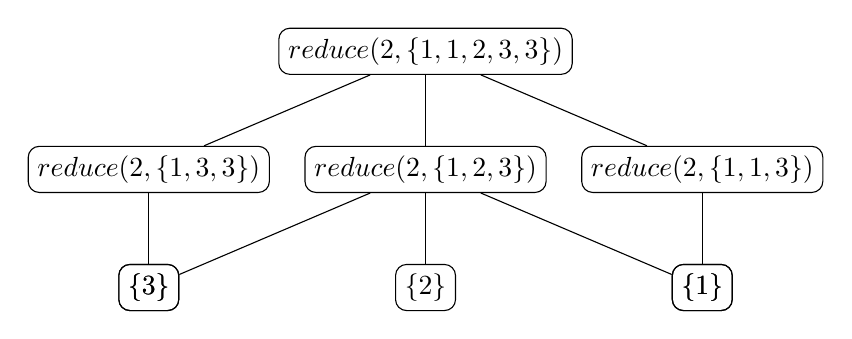
\begin{tikzpicture}[sibling distance=10em,
        every node/.style = {shape=rectangle, rounded corners,
        draw, align=center}]
        \node {$reduce(2, \{1, 1, 2, 3, 3\})$}
            child { node {$reduce(2, \{1, 3, 3\})$}
                child { node {$\{3\}$} }
            }
            child { node {$reduce(2, \{1, 2, 3\})$} 
                child { node {$\{3\}$} }
                child { node {$\{2\}$} }
                child { node {$\{1\}$} }    
            }
            child { node {$reduce(2, \{1, 1, 3\})$}
                child { node {$\{1\}$} }
            };
    \end{tikzpicture}
    \caption{Recursive Descend of \emph{reduce()}}
    \label{fig:Reduce}
    \end{figure} 
\end{example}

The correctness of the Misra-Gries algorithm is based on the generalized pairing argument, formalized in the following theorem.

\begin{theorem}[{\cite[Theorem 1]{Misra_1982}}]
    \label{th:Pairing}
    Given a multiset $A$ containing $m$ elements. Only elements in $reduce(k+1, A)$ may occur more than $\frac{m}{k+1}$ times in $A$.  
\end{theorem}

\begin{proof}
    Let $A$ be a multiset containing $m$ elements. Deleting $k+1$ elements from $A$ can be done for a maximum of $\frac{m}{k+1}$ times, since $|A| < k+1$ after the $\frac{m}{k+1}$-th deletion. The number of distinct elements $e$ in $A$ is always less or equal to the number of total items in $A$:
    
    \begin{equation}
        \label{eq:PairingProof}
        |support(A)| = HH\left(\frac{1}{m+1}, A\right) \leq |A| < k+1
    \end{equation}

    $reduce()$ stops and returns a reduced multiset if Equation~\ref{eq:PairingProof} is true. Any element left in $R = reduce(k + 1, A)$ has been deleted between $0$ and $\frac{m}{k + 1}$ times. Therefore an element in $R$ can have a frequency $_e$, where $1 \leq f_e \leq m$, but any element that was deleted through $reduce()$ cannot have a frequency above $\frac{m}{k + 1}$. Thus, for any multiset $A$, there is no $e$ in $A$ such that $e$ is in $reduce(k+1, A)$ and $f_e > \frac{m}{k + 1}$.
\end{proof}

The original algorithm given by Misra and Gries \cite[Algorithm 3]{Misra_1982} makes direct use of Definition~\ref{def:Reduce} and Theorem~\ref{th:Pairing} and is described in detail as Algorithm~\ref{alg:OriginalMisraGries} given below. The Misra-Gries algorithm solves both the frequency estimation subproblem and the \textsc{Frequent} problem at the same time. The multiset $D$, that is returned by the Misra-Gries algorithm, holds an approximate solution to the \textsc{Frequent} problem. The estimated set of frequent items $HH^*$ is given as the set of distinct elements $support(D)$ and the multiplicity of an element $e$ in $D$ represents the frequency estimate $f_e^*$.

The \textsc{Frequent} problem expects the $k$ most frequent distinct elements $e$ from a stream $S$. The relative error $\varepsilon$ of the estimated solution is controlled by $k$, such that $\varepsilon = \frac{1}{k + 1}$. This is derived from the following intuition: The higher $k$ the more counts of elements $e$ have to be estimated. This uses more space and thus keeps more information, which in turn reduces the chance for an error. More formally the bounds for $f_e^*$ are given in Theorem~\ref{th:MisraGries}.

\begin{theorem}[{\cite[Theorem 1.3.1]{Chakra2020}}]
    \label{th:MisraGries}
    Let $e$ be an arbitrary token in $[n]$ and let $k > 0$ be a constant integer. The \hyperref[alg:OriginalMisraGries]{Misra-Gries algorithm} provides an estimate $f_e^*$ of the true value $f_e$, satisfying 
    
    \begin{equation*}
        f_e - \frac{m}{k+1} \leq f_e^* \leq f_e.
    \end{equation*}
\end{theorem}

\begin{proof}
The upper and the lower bound can be proved separately.

Case $f_e^* \leq f_e$: The multiplicity of $e$ is increased if and only if the stream's current item $s_i$ matches $e$. Hence an increase to the true frequency $f_e$ of one will deterministically cause an increase of one in the estimated frequency $f_e^*$.

Case $f_e^* \geq f_e - \frac{m}{k + 1}$: An error in the estimation may only occur when $|support(D)| > k$, since this would invoke $reduce()$. If an element $e$ in $D$ had, at one point, a multiplicity $\bm{m}_D(e) > 0$ and this $\bm{m}_D(e)$ was later decremented by the algorithm but remained above zero, $\bm{m}_D(e) = f_e^*$ deviates from the true total frequency $f_e$. This is because $\bm{m}_D(e)$, at this point, represents the relative frequency of $e$ in comparison to other frequent items. This relative frequency is obtained solely by decrementing by one for a maximum of $\frac{m}{k+1}$ times.

Put together this satisfies Definition~\ref{def:RelaxedHH} and proves Theorem~\ref{th:MisraGries}.
\end{proof}

\begin{algorithm}
    \caption{The original Misra-Gries algorithm}
    \label{alg:OriginalMisraGries}
    \DontPrintSemicolon
    \KwData{Updates $s_i$ to stream $S$ with $i \in [m]$} 
    \KwResult{A multiset $D$ of elements $e$ with $f_e^* > \frac{m}{k+1}$; A counter $c_d = |support(D)|$}
    $c_d \gets 0$ \;
    $D \gets \{\}$ \tcp*{Initialize $D$ as a empty set}
    \For{$i \gets 1$ \KwTo $m$}{
        \If{$s_i \notin D$}{
            $D \gets D \cup s_i$ \;
            $c_d \gets c_d + 1$ \;
            \If{$c_d = k+1$}{ 
                $D \gets reduce_1(k+1, D)$ \tcp*{Delete $k+1$ distinct occurences}
                $c_d \gets |support(D)|$ \tcp*{Update $c_d$ accordingly}
            }
        }\ElseIf(\tcp*[f]{$s_i$ is not distinct in $D$}){$s_i \in D$}{
            $D \gets D \cup s_i$ \;
        }
    }
    \Return{$D, \ c_d$}
\end{algorithm}

The analysis of this algorithm requires the definition of the AVL data structure.

\begin{definition}[Georgy Adelson-Velsky \& Evgenii Landis, 1962]
    \label{def:AVL}
    A AVL tree is a data structure named after its inventors Georgy Adelson-Velsky and Evgenii Landis.
    
    The basic tree $T$ is defined as $T = (V, E)$ where $V$ is a set of vertices or nodes $v \in V$ and $E$ is a set of edges $e \in E$ between two vertices $v_1$ and $v_2$, given as $e = (v_1, v_2)$. An edge describes a relation between a parent node $v_1$ and a child node $v_2$. Nodes can contain either a single key or a tuple of a key and an additional value. A root node $r$ has no parents, i.e.,
    \[\forall v \in V \ \nexists e \in E \colon e = (v, r)\]
    while a leaf node $f$ has no children, such that
    \[\forall v \in V \ \nexists e \in E \colon e = (l, v).\] 
    The height of a tree $h(T)$ is then given as the longest path between the root node $r$ and a leaf $l$. A path $P(r, l) = v_1 , \dots , v_{i-1}, v_i$ is a sequence of nodes where $r = v_1$ and $l = v_i$ and every consecutive two nodes share an edge:
    \[\forall v_j \in P(r,l) \ \exists e \in E \colon e = (v_j, v_{j+1}).\]
    
    A tree $T$ is a AVL tree if the following conditions are fulfilled:
    \begin{itemize}
        \item[-] $T$ is a \emph{binary tree}: Every node $v \in V$ has a maximum of two children.
        \item[-] $T$ is a \emph{binary search tree}, i.e., for every given node $v \in V$ contains the left subtree only keys that are smaller than all keys contained in the right subtree.
        \item[-] For every node $v \in V$: The difference of the left subtrees height and of the right subtrees height is the $v$'s balance factor $BF(v)$ and $|BF(v)| \leq 1$.     
    \end{itemize}  
\end{definition}

\begin{analysis}
    Misra and Gries \cite[Chapter 4]{Misra_1982} implement the multiset $D = (support(D), \bm{m}_D)$ as an AVL tree with $c_d = |support(D)| = k+1$ nodes. Each node $j$, with $1 \leq j \leq k+1$, is a tuple $(v_j, c_j)$ where $v_j$ in $support(D)$ is the value of an distinct element in $D$ and $c_j = \bm{m}_D(v_j)$ is its multiplicity. This takes $\lfloor \log n \rfloor + 1$ space for each value $v_j$ and $\lfloor \log m \rfloor$ + 1 for each counter $c_j$. Since there are at most $k$ distinct elements in the result, the total space is $O(k \cdot (\log (m) + \log (n)))$.

    Ensuring that all conditions of an AVL tree are maintained throughout the insertion and deletion of nodes is called self balancing. This requires time to compute but allows for searching, inserting and deleting elements in $O(\log k)$ worst-case time. The time required for rebalancing the tree once necessary is constant and can therefore be attributed to the inserting and deleting operations without altering their time complexity class.   

    The algorithm's runtime is dominated by the operations on $D$. For every item $s_i$ in the input stream $S$ the condition $s_i \in D$ needs to be checked. This requires searching the AVL tree representation of $D$. Since $D$ holds a maximum of $k+1$ nodes a single search needs $O(\log k)$. 

    If $|support(D)| < k+1$ and $s_i$ is not in $D$ one element has to be inserted into the tree. This is done in $O(\log k)$. If, on the other hand $|support(D)| = k+1$ and $s_i \notin D$, $reduce_1(k+1, D)$ is invoked decrementing $k+1$ elements in constant time and deleting a maximum of $k+1$ elements in $O(k \cdot \log k)$ total time.

    This yields a per item processing time of $time_{proc} = O(k \cdot \log k)$ in the worst case and an amortized $time_{comp} = O(\frac{m}{k} \cdot k \cdot \log k) = O(m \cdot \log k)$ since this reduction may occur maximally $\frac{m}{k+1}$ times over a stream of length $m$.
\end{analysis}

A trivial second pass over the data would solve \textsc{Frequent} exactly by calculating $f_d$ for every distinct element $d$ in $support(D)$ and delete every $d$ from the solution where $f_d < \frac{m}{k}$. The time and space complexity remain the same for this extended Misra-Gries algorithm as was the case for the original algorithm.


\subsection{Modified Misra-Gries by Karp et~al.}
\label{subsec:ModifiedMisraGries}

The core information needed for solving \textsc{Frequent} is a set of distinct values and their respective frequencies. In the original algorithm given by Misra and Gries \cite{Misra_1982} these values were kept in a multiset. A multiset can be implemented as an AVL tree and allows for efficient search, insert, and delete operations -- all done in logarithmic time depending on the tree's size.   

Karp et~al. \cite{Karp2003} modify the original account by using a map instead of a set data structure. A map $M$ represents a number of associations between a set of keys as $keys(M)$ and their values $M[l]$ with $l$ in $keys(M)$. Here, the distinct values are keys to their respective frequencies as values. This results slight modifications yields Algorithm~\ref{alg:ModifiedMisraGries}. A graphical overview of the data structures used both in the original and the modified Misra-Gries algorithm is given in Figure~\ref{fig:MisraGriesData}.

\begin{algorithm}
    \caption{Modified Misra-Gries Algorithm by Karp et~al.\label{alg:ModifiedMisraGries}}
    \DontPrintSemicolon
    \KwData{Updates $s_i$ to stream $S$ with $i \in [m]$} 
    \KwResult{A map $M$ with $keys(M)$ as elements $e$ with $f_e^* > \frac{m}{k+1}$ and $M[e] = f_e^*$ as the value to key $e$}
    $M \gets \{\}$ \tcp*{Initialize $M$ as an empty map}
    \For{$i \gets 1$ \KwTo $m$}{
        \If{$s_i \in keys(M)$}{
            $M[s_i] \gets M[s_i] + 1$ \;
        }\Else(\tcp*[f]{Initialize a new key-value pair, since $s_i \notin keys(M)$}){
            $keys(M) \gets keys(M) \cup s_i$ \;
            $M[s_i] \gets 1$ \;
        }
        \If(\tcp*[f]{Keep at most $k$ key-value pairs in $M$}){$|keys(M)| > k$}{
            \ForEach{$l \in keys(M)$}{
                $M[l] \gets M[l] - 1$ \;
                \If{$M[l] = 0$}{
                    $keys(M) \gets keys(M) \setminus l$ \tcp*{Remove $l$ from $M$}
                }
            }
        }
    }
    \Return{$M$}
\end{algorithm}

\begin{definition}[Hash table, based on Knuth {\cite[Chapter 6.4]{Knuth1998}}]
    \label{def:HashTable}
    Given a hash function $h: L \to I$ that maps keys $l \in L$ to hash values $i \in I$ and where $|L| \leq |I|$.

    A hash table $HT$ is a data structure combining hash functions and a strategy for collision resolution. A \emph{collision} occurs if $l_1 \neq l_2$ and $h(l_1) = h(l_2)$. The memory space of $HT$ is partitioned into individually addressable buckets. These buckets hold any amount of key-value pairs $(l, v)$ and are accessible at $h(l)$. The collision resolution states how multiple entries in a bucket are represented, for example as a linked list.
\end{definition}

$M$ is implemented as a hash table. This yields space in $O(k)$ and improves the per item processing time to an \emph{amortized} $time_{proc} = O(1)$ according to Karp et~al. \cite[Theorem 2.2 and adjoining proof]{Karp2003}. The authors argue that for each received item $s_i$ only a constant number of operations are needed if no deletions occur, i.e., while the number of key-value pairs in $M$ is below or equal to $k$. In this case the condition $s_i \in keys(M)$ needs to be checked, which due to $M$'s implementation as a hash table is done in \emph{amortized} $O(1)$. If deletions occur, the time required could be attributed to the original items processing time, since only items added as keys may be deleted later on, thus retaining \emph{amortized} constant time.      

\begin{example}
    \label{ex:MisraGriesData}
    Let $E = \{1, 1, 2, 3, 1, 2, 2, 3, 1, 2\}$ be a multiset. Following Definition~\ref{def:multiset}, this can be represented as a 2-tuple $E = (support(E), \bm{m}_E)$ consisting of the set of distinct elements $support(E) = \{1, 2, 3\}$ and a vector of the frequency, also called the multiplicity, for each of these elements as
    \[
        \bm{m}_E = 
        \begin{pmatrix}
            m_E(1) \\
            m_E(2) \\
            m_E(3)
        \end{pmatrix}
        =
        \begin{pmatrix}
            4 \\
            4 \\
            2
        \end{pmatrix}
        .
    \]
    The sum of all individual frequencies is equal to the total number of elements in $E$ denoted as $|E|$:
    \[\sum_{e \in [3]} m_E(e) = |E|. \]
    
    In the original Misra-Gries algorithm an AVL tree is used to store this information while the algorithm modified by Karp makes use of a hash table. The following is a graphical illustration of these two data structures representing the multiset $E$.
    
    \captionsetup{type=figure}
    \begin{center}
    \begin{minipage}{.45\textwidth}
    \centering
    \begin{tikzpicture}[
        >=stealth,
        ln/.style={rectangle split,rectangle split parts=2,rectangle split horizontal,draw,rounded corners},
        en/.style={inner sep=2pt},
        dt/.style={circle,fill,minimum size=1.5mm,inner sep=0pt},
        ht/.style={rectangle split,rectangle split parts=5,draw,rounded corners}
        ]
        % hashtable
        \node (ht) [ht,inner sep=8] {};
        %% coordinates
        \path let \p1=(ht.text east), \p2=(ht.center) in coordinate (h1) at (\x2,\y1);
        \path let \p1=(ht.four east), \p2=(ht.center) in coordinate (h2) at (\x2,\y1);
        \path let \p1=(ht.two east), \p2=(ht.center) in coordinate (h3) at (\x2,\y1);
        %% lists - this could be a for loop
        %%% h1
        \node[ln] (h1') [right of=h1,node distance=1.5cm] {$4$\nodepart{two}} edge [<-] (h1);
        \coordinate (h1'2) at (h1'.two south |- h1'.two east);
        \node[en] (h1'') [right of=h1',node distance=1.5cm] {$\varnothing$} edge [<-,dashed] (h1'2);
        \node[dt] at (h1) {};
        \node[dt] at (h1'2) {};
        \node [left=0.85cm of ht.text,anchor=base] {$h(1)$};
        %%% h2
        \node[ln] (h2') [right of=h2,node distance=1.5cm] {$4$\nodepart{two}} edge [<-] (h2);
        \coordinate (h2'2) at (h2'.two south |- h2'.two east);
        \node[en] (h2'') [right of=h2',node distance=1.5cm] {$\varnothing$} edge [<-,dashed] (h2'2);
        \node[dt] at (h2) {};
        \node[dt] at (h2'2) {};
        \node [left=0.85cm of ht.four,anchor=base] {$h(2)$};
        %%% h3
        \node[ln] (h3') [right of=h3,node distance=1.5cm] {$2$\nodepart{two}} edge [<-] (h3);
        \coordinate (h3'2) at (h3'.two south |- h3'.two east);
        \node[en] (h3'') [right of=h3',node distance=1.5cm] {$\varnothing$} edge [<-,dashed] (h3'2);
        \node[dt] at (h3) {};
        \node[dt] at (h3'2) {};
        \node [left=0.85cm of ht.two,anchor=base] {$h(3)$};
        %% label
        \node [above=0.3cm of ht.north,anchor=south] {Hashtable};
    \end{tikzpicture}
    \end{minipage}
    \begin{minipage}{.45\textwidth}
    \centering
    \begin{tikzpicture}[
        tn/.style={rectangle split,rectangle split parts=2,rectangle split horizontal,draw,rounded corners},
        en/.style={inner sep=2pt},
        level 2/.style={sibling distance=2em},
        edge from parent/.style={draw,-stealth}
        ]
        % AVL tree
        \node[tn] (root) {2\nodepart{two}4}
            child{ node[tn] {1\nodepart{two}4}
                child{ node[en] {$\varnothing$} edge from parent [dashed]}
                child{ node[en] {$\varnothing$} edge from parent [dashed]}
                }
            child{ node[tn] {3\nodepart{two}2}
                child{ node[en] {$\varnothing$} edge from parent [dashed]}
                child{ node[en] {$\varnothing$} edge from parent [dashed]}
                };
        % label
        \node [above=0.3cm of root.north,anchor=south] {AVL tree};
    \end{tikzpicture}
    \end{minipage}
    \end{center}
    \captionof{figure}{Data Representation and Structure in the Misra-Gries Algorithm \label{fig:MisraGriesData}}
\end{example}

The exact runtime of operations on a hash table depends on their concrete implementation, i.e., the choice of hash function and the collision resolution. Nevertheless, it can be regarded to be $O(1)$ on average for searching, inserting and deleting. Searching $HT$ for $(l, v)$ is described in Algorithm~\ref{alg:HT}, due in part to Knuth's Algorithm C \cite[p.~521]{Knuth1998}:

\begin{algorithm}
    \caption{Searching a Hash Table\label{alg:HT}}
    \DontPrintSemicolon
    \KwData{A key $\mathcal{K}$, a hash function $h()$, and a hash table $HT$} 
    \KwResult{A associated value $v$, or $\bot$ if $l \notin HT$}
    \nl $i \gets h(l)$ \tcp*{Computing $HT$'s index by hashing}
    \nl \If{$HT(i) \neq \varnothing$}{
        \nl \ForEach(\tcp*[f]{All possible entries at $HT(i)$}){$(l, v)$ as $e \in HT(i)$}{
            \nl \If(\tcp*[f]{Compare the entries key with the input key}){$\mathcal{K} = e[0]$}{
                \nl \Return{$e[1]$}
            }
        }
    }
    \nl \Return{$\bot$}
\end{algorithm}

The runtime of Algorithm~\ref{alg:HT} is dominated by the runtime of the hash function $h$ in line 1 to compute the index $i$ and by the for loop, iterating over all possible values in bucket $HT(i)$, in line 3. The hash functions time complexity can be considered constant, but the number of operations required in the for loop depend on $HT$'s load factor $\alpha$ and probability. The load factor is $\alpha = \frac{k}{B}$ with $k$ being the maximum number of reported elements as usual and $B$ being the number of buckets in $HT$, i.e., 
\[h(l) = i \colon l \in [k] \text{ and } i \in [B].\]   
With $HT$ in $O(k)$ there are $k$ buckets resulting in $\alpha = 1$. In theory there would be enough buckets to assign exactly one key-value pair $(l, v)$ to one bucket but this assignment is done via $h()$ and is therefore probabilistic. There are no hash functions guaranteeing collision free operation and hence buckets with multiple entries in a bucket have to be accounted for. In fact, the worst case performance happens if all keys $l \in [k]$ are mapped to the same $h(l) = i$. Then the worst case time complexity for processing individual items $s_i$ becomes dependent on $k$. If a singly linked list is chosen as the collision resolution, $time_{proc}$ is in $O(k)$ in the worst case -- worse than the AVL trees guaranteed $O(\log k)$.

The algorithm stores $k$ elements and their respective counter. Once there are more distinct items in $S$ than there are buckets in $HT$, i.e., 
\[\left| HH \left(\frac{1}{k + 1}, S \right) \right| > B \text{ with } k = m = |support(S)|\]
the counters for $k$ elements need to be decremented and deleted from $HT$ if the decremented counter is zero. To reduce the \emph{amortized} processing time in $O(1)$ to \emph{expected} worst-case constant time Karp et~al. \cite[p.~54]{Karp2003} augment a hash table with a doubly linked list $\mathcal{L}$ holding every $l \in k$ and a linked list $\mathcal{V}$ holding their respective counts. This reduces the complexity during deletion to transforming a pointer from an $l \in \mathcal{L}$ to a $v \in \mathcal{V}$. This structure is detailed in Figure~\ref{fig:KarpConstant} using the same data as in \hyperref[ex:MisraGriesData]{first Example}. 

\begin{figure}
    \centering
    \begin{tikzpicture}[
        >=stealth,
        dln/.style={rectangle split,rectangle split parts=4,rectangle split horizontal,draw,rounded corners, inner sep=4},
        sln/.style={rectangle split,rectangle split parts=3,rectangle split horizontal,draw,rounded corners, inner sep=4},
        en/.style={inner sep=2pt},
        dt/.style={circle,fill,minimum size=1.5mm,inner sep=0pt},
        ht/.style={rectangle split,rectangle split parts=5,draw,rounded corners, inner sep=8}
        ]
        % hashtable
        \node[ht] (ht) {};
        %% coordinates
        \path let \p1=(ht.three east), \p2=(ht.center) in coordinate (h1) at (\x2,\y1);
        \path let \p1=(ht.four east), \p2=(ht.center) in coordinate (h2) at (\x2,\y1);
        \path let \p1=(ht.five east), \p2=(ht.center) in coordinate (h3) at (\x2,\y1);
        %% labels
        \node [left=0.85cm of ht.three,anchor=base] {$h(1)$};
        \node [left=0.85cm of ht.four,anchor=base] {$h(2)$};
        \node [left=0.85cm of ht.five,anchor=base] {$h(3)$};
        %% dots
        \node[dt] at (h1) {};
        \node[dt] at (h2) {};
        \node[dt] at (h3) {};
        
        % doubly linked list
        \node[dln] (k1) [right=2cm of ht.two east] {\nodepart{two}$1$};
        \node[dln] (k2) [right=0.5cm of k1] {\nodepart{two}$2$};
        \node[dln] (k3) [right=0.5cm of k2] {\nodepart{two}$3$};
        \node[en] (k1') [left=0.5cm of k1] {$\varnothing$} edge [<-,dashed] (k1.mid);
        \node[dt] at (k1.mid) {};
        \node[en] (k3') [right=0.5cm of k3] {$\varnothing$} edge [<-,dashed] (k3.four south |- k3.mid);
        \node[dt] at (k3.four south |- k3.mid) {};
        %% links
        \draw[->,rounded corners] (h1) -- (k1.two south |- h1) -- (k1.two south);
        \draw[->,rounded corners] (h2) -- (k2.two south |- h2) -- (k2.two south);
        \draw[->,rounded corners] (h3) -- (k3.two south |- h3) -- (k3.two south);
        %% first step
        \draw[->,thick,red] ($(k1.four south |- k1.mid)+(0,1mm)$) to[bend left=30] ($(k2.mid)+(0,1mm)$);
        \node[dt,red] at ($(k1.four south |- k1.mid)+(0,1mm)$) {};
        \draw[<-,thick,blue] ($(k1.four south |- k1.mid)-(0,1mm)$) to[bend right=30] ($(k2.mid)-(0,1mm)$);
        \node[dt,blue] at ($(k2.mid)-(0,1mm)$) {};
        %% second step
        \draw[->,thick,red] ($(k2.four south |- k2.mid)+(0,1mm)$) to[bend left=30] ($(k3.mid)+(0,1mm)$);
        \node[dt,red] at ($(k2.four south |- k2.mid)+(0,1mm)$) {};
        \draw[<-,thick,blue] ($(k2.four south |- k2.mid)-(0,1mm)$) to[bend right=30] ($(k3.mid)-(0,1mm)$);
        \node[dt,blue] at ($(k3.mid)-(0,1mm)$) {};
        
        % singly linked list
        \node[sln] (v1) [above=2cm of k1.mid] {\nodepart{two}$2$};
        \node[sln] (v2) [right=0.5cm of v1] {\nodepart{two}$4$};
        \node[en] (v2') [right=0.5cm of v2] {$\varnothing$} edge [<-,dashed] (v2.three south |- v2.mid);
        \node[dt] at (v2.three south |- v2.mid) {};
        %% links
        \draw[->,thick,red] (v1.three south |- v1.mid) -- (v2.mid);
        \node[dt,thick,red] at (v1.three south |- v1.mid) {};
        %% keys
        \draw[->] (k1.three south |- k1.mid) -- (v2.two south);
        \node[dt] at (k1.three south |- k1.mid) {};
        \draw[->] (k2.three south |- k2.mid) -- (v1.two south);
        \node[dt] at (k2.three south |- k2.mid) {};
        \draw[->] (k3.three south |- k3.mid) -- (v2.two south);
        \node[dt] at (k3.three south |- k3.mid) {};
        
        % Label
        \node [above=0.3cm of ht.north,anchor=south] {HT};
        \node [right=0.3cm of v2'.east,anchor=west] {$\mathcal{V}$};
        \node [right=0.3cm of k3'.east,anchor=west] {$\mathcal{L}$};
        
    \end{tikzpicture}
    \caption{Data Representation for the Modified Misra-Gries Algorithm \label{fig:KarpConstant}} 
\end{figure}

\begin{analysis}
    The accuracy of the modified algorithm is the same as the original one. An approximation $HH_{\varepsilon}$, where the relative error $\varepsilon$ is controlled by $k = \frac{1}{\varepsilon}$, can be provided in a single pass but an exact solution requires two passes. 
    
    Since the selection and deletion operation are extensions of the search operation of Algorithm~\ref{alg:HT} the time complexity is $time_{proc} = O(1)$ and $time_{comp} = O(m)$ for both single pass and dual pass operations as per Karp et~al. \cite[Theorem~2.2 and Corollary~2.3]{Karp2003}. Since these time bounds include hashing operations their actual time requirements are highly dependent.   
\end{analysis}


\section{Frequency Moments}
\label{sec:FrequencyMoments}

Frequency moments are an important metric about a stream's data. They are also convenient for the main focus of this thesis -- the general \textsc{Frequent} problem and its solution. The connections of these two topics is established in the following definition.

\begin{definition}[{\cite[Introduction]{Alon1999}}]
    \label{def:FM}
    Given a stream $S$ as a sequence of items $s_i$ with $i \in [m]$ and $s_i \in [n]$. The frequency of a given  element $s_i$ is the cardinality of the set of indices $j \in [m]$ such that $s_i = s_j$ yielding
    \[f_i = \left| \{j \mid s_j = i\}\right| \text{, for all } i \in [n] \text{ and } j \in [m]. \] 
    The $k$-th frequency moment of $S$ is defined as
    \[F_k(S) = \sum_{i=1}^{n} f_i^k. \]
\end{definition}

The concept of frequency moments was first introduced by Alon, Matias and Szegedy \cite[p.~2]{Alon1999}. According to the authors, frequency moments provide useful statistics on a set such as the degree of \emph{skew} in the data. This information is of particular interest in database applications. Values like the number of distinct elements in a relation and estimates of join sizes are used in database query optimization, as pointed out by Chakrabarti \cite[Section~6.1]{Chakra2020}. 

$F_k$ is defined for every real $k > 0$. Let $\bm{f} = f(S) = (f_1, f_2, \ldots, f_n)$ be a vector of each elements frequency in the stream. $F_1$ is the sum of all frequencies and hence the length of stream $S$ as $F_1 = \sum_{i} f_i = m$. This is equivalent to the cardinality $|S|$ when viewing $S$ as a multiset as the sum of every distinct elements $e$ multiplicity in $S$. With $cs = support(S)$ this yields
\[F_1 = \sum_{i \in [n]} f_i = m = \sum_{e \in cs} m_S(e) = \left| S \right| .\]
The exact value of $F_1$ can be obtained by maintaining a single binary counter, consuming $\Theta(\log m)$ bits of space. 

The second frequency moment is the dot product of $\bm{f}$ with itself. This value is referred to as the \emph{repeat rate} or \emph{Gini's index of homogeneity} by Alon et~al. \cite[p.~1]{Alon1999} and is used in computing the \emph{surprise index} $SI$, as described by Good \cite[p.~90]{Good1989}. As a relation between the probability of a specific realization of a random variable $P(R = r)$ and the expected value of that variable $E(R)$ as
\[SI = \frac{E(R)}{P(R = r)},\]
this index formalizes how much of a \emph{surprise} the realization of $R$ as $r$ is. A realization $r$ should be expected if $SI$ is close to one. A high value for $SI$ on the contrary means $P(R = r)$ is small, making $r$ a rare occurrence, as well as that there are other realizations with far higher probabilities. The frequencies of elements $e$ in $S$ contained in $\bm{f}$ are absolute while the probability of their occurrence $P(S = e)$ is relative to the total number of occurrences. This number is equal to the length of the stream and given in this model as $\sum_i f_i = m$. Analogous to $\bm{f}$ a vector of probabilities $\bm{p}$ is derived by 
\[\bm{p} = (p_1, p_2, \ldots, p_n) = \left( \frac{f_1}{m}, \frac{f_2}{m}, \ldots, \frac{f_n}{m} \right) = \frac{1}{m} \bm{f}.\] 
The expected value for the frequency of an element occurring in $S$ is then the sum of all frequencies weighted by their respective probability
\[E(\bm{f}) = \sum_{i=1}^n p_i f_i = \sum_{i=1}^n \frac{f_i}{m} f_i = \frac{1}{m} \sum_{i=1}^n f_i^2 = \frac{1}{m} F_2(S).\] 
This allows for a more intuitive interpretation of the second frequency moment where $F_2$ is an absolute measure of a sequence's frequencies that is closely related to the relative expected value of its frequencies. $F_2$ does not require $m$ which is beneficial in the streaming scenario where $m$ might be infinite or unknown. Setting $m = i$ for each update $s_i$ is unfeasible if $i$ is very large and $\log i$ exceeds a memory limit or at least computation intensive since $\bm{p}$ needs to be re-computed after every update $s_i$. The \emph{surprise index} of a stream's frequencies is identical whether the expected value, and therefore $m$, or the second frequency moment is used in its computation:      
\[SI_i = \frac{E(\bm{f})}{p_i} = \frac{\frac{1}{m} F_2(S)}{\frac{f_i}{m}} = \frac{F_2(S)}{f_i}.\]

$F_0$ is the number of distinct elements in $S$. It is derived from Definition~\ref{def:FM} and the convention of $0^0 \coloneqq 0$ so that $F_0$ is incremented by one only if $f_i > 0$. When viewing $S$ as a multiset, $F_0$ is equivalent to the cardinality of $support(S)$ with
\[F_0 = \sum_i f_i^0 = \left| \{e \in U \mid e \in S \text{ and } f(e) > 0\} \right| = support(S).\]


\section{Estimating the Number of Distinct Elements}
\label{sec:DistinctEstimation}

This section is concerned with estimating the number of distinct elements in a stream also called $0$-th frequency moment. $F_0$ is just the quantity of those elements and contains neither the element itself nor any additional information on them. Regardless, maintaining $F_0$ provides valuable insights in a number of scenarios. One of which is laid out in detail as motivation below.
  
The set of distinct elements $D$ of a stream $S$ could theoretically be computed using the Misra-Gries algorithm discussed in Section~\ref{subsec:MisraGries}. This would mean setting the maximum number of returned items $k$ to the length of the stream $m$ since, with the streams elements being drawn from a universe $U$ with $|U| = n > m$ and no element occurring more than once follows that $|D| = m$. The space requirements of this algorithm are however linear with regards to $k$, hence exceeding the sublinear space requirement for $k=m$ and a large $D$. Choosing a smaller $k$ reduces the required space but opens the possibility of not including all distinct elements in the returned set. Keeping an estimate of $F_0$ while maintaining $k$ Misra-Gries counters would ensure that $D$ contains every distinct element as long as $F_0 \leq k$. If that is not the case, this information may be used to decide if the available memory to the Misra-Gries algorithm could be extended or if the algorithm should be kept as is and its result be interpreted accordingly. 

This problem is called \textsc{Distinct-Elements} by Chakrabarti \cite[Section 2.1]{Chakra2020}. It is stated there that this problem cannot provably be solved exactly and deterministically in sublinear space. We shall therefore focus on providing an $(\varepsilon, \delta)$-estimate of $F_0$ where there are random elements in the algorithm, thus $\varepsilon, \delta > 0$. 


\subsection{The Tidemark Algorithm} 
\label{subsec:Tidemark}

The algorithm discussed here is originally due to Flajolet and Martin \cite[Section~2]{Flajolet1985} and was later modified by Alon et~al. \cite[Section~2.3]{Alon1999}. It is called the Tidemark algorithm by Chakrabarti \cite[Section~2.2]{Chakra2020} and allows for an introduction to two important techniques in data stream processing -- universal hashing and the median trick.

\begin{definition}[random variables]
    A set of random variables $\{X_1, \ldots, X_l\}$ is $k$-independent if
    \[ Pr \left[ \bigcap_{i \in J} X_i = x_i \right] = \prod_{i \in J} Pr \left[ X_i = x_i \right] \]
    holds for every subset $J \subseteq [l]$ with $|J| \leq k$ and every realization $x_i$. 
\end{definition}

\begin{definition}[{\cite[Section~2, Exercises]{Chakra2020}}]
    \label{def:uniHash}
    Let $X$ and $Y$ be finite sets and let $\mathcal{H}$ be a family of functions such that $\mathcal{H} = \{h \mid h \colon X \mapsto Y\}$. Let further $h \sim_R \mathcal{H}$ denote that $h$ is being chosen uniformly and randomly from $\mathcal{H}$. 

    Two conditions must hold for $\mathcal{H}$ to be $k$-universal. 
    \begin{itemize}
        \item[-] The random variable $h(x)$ is uniformly distributed in $Y$ for every $x$ in $X$. 
        \item[-] A set of $k$ hashed values $\{h(x_1), \ldots, h(x_k)\}$ is $k$-independent given a set of $k$ values $\{x_1, \ldots, x_k\}$ where for all $i, j$ in $[k]$, $i \neq j$ implies $x_i \neq x_j$. 
    \end{itemize}
\end{definition}

For this section $2$-universal families of hash functions are of particular interest. With $h$ randomly chosen from such a family the values of $h(x)$ are uniformly distributed in $Y$ for all $x \in X$ and the probability of a specific realization $Pr \left[ h(x) = y \right] = \frac{1}{|Y|}$ , with $y \in Y$, is independent from another, second realization. This reduces the probability for collisions, i.e., $h(x_1) = h(x_2)$ for all $x_1, x_2 \in X$ with $x_1 \neq x_2$. Definition~\ref{def:uniHash} implies that this probability, for all $y_1, y_2 \in Y$, is
\[Pr \left[ h(x_1)=y_1 \cap h(x_2) = y_2 \right] = \frac{1}{|Y|^2}.\]
This applies for $y_1 = y_2$ or $y_1 \neq y_2$ regardless.

\begin{example}
    Given a prime number $p$ and two random numbers $a, b \in [p]$, then $\mathcal{H} \coloneqq \{h(x) = a \cdot x + b \bmod p\}$ is a 2-universal family of hash functions.
\end{example}

The Tidemark algorithm given in Algorithm~\ref{alg:Tidemark} works as follows. Every update $s_i$ is hashed via $h \sim_R \mathcal{H}$ and the resulting values $h(s_i)$ are then considered to be uniformly distributed in $[n]$. A helper function $zeros()$ is applied in order to retrieve the number of trailing zeros of the binary representation of $h(s_i)$. More formally, $zeros(p)$ is defined for every $p > 0$ as
\[zeros(p) = max( \{ l \mid 2^l \text{ divides } p\} ).\]
The maximal value of $zeros(h(s_i))$ for all $i$ in $[m]$ is maintained in $z$ as the maximal number of trailing zeros over all hash values. With $F_0(S)$ being the number of distinct values in $S$, $z$ is used as an approximation for $F_0(S)$'s binary representations length in bits. This value is converted to decimal with $2^{z + \frac{1}{2}}$ and returned.

\begin{algorithm}
    \caption{The Tidemark algorithm by Alon et~al.\label{alg:Tidemark}}
    \DontPrintSemicolon
    \KwData{Updates $s_i$ to stream $S$ with $i \in [m]$ and $s_i \in [n]$} 
    \KwResult{$2^{z + \frac{1}{2}}$ as an estimate for $F_0$}
    Choose random $h \colon [n] \mapsto [n]$ \;
    $z \gets 0$ \;
    \For{$i \gets 1$ \KwTo $m$}{
        \If{$zeros(h(s_i)) > z$}{
            $z \gets zeros(h(s_i))$ \;
        }
    }
    \Return{$2^{z + \frac{1}{2}}$}
\end{algorithm}

The algorithm's functioning is not apparent since the number of distinct elements is limited by the length of the stream, i.e., $1 \leq F_0 \leq m$ if $n \gg m$ is assumed, while the number of trailing zeros is a function of the size of the universe $n$ with values in $\{0, 1, \ldots, \left\lfloor \log (n - 1) \right\rfloor \}$. The intuition is rather based on a scarcity argument. The streams updates are mapped uniformly to $[n]$ after hashing. This means that the probability of $h(s_i)$ being a specific value is $\frac{1}{n}$, hence only depending on $n$ and the same for all $s_i$. The probability of $zeros(h(s_i))$ realizing as a specific value on the other hand is inversely proportional to that value. This is exemplified with the following cases. 

A value of zero for $zeros(p)$ means that there are no trailing zeros. This is equal to the last bit of $p$'s binary representation being a $1$ which in turn applies to every uneven number in $[n]$. Since every other number in $[n]$ is uneven the probability of $zeros(p) = 0$ is $\frac{1}{2}$. With every even number having at least one trailing zero the same argument applies here, yielding $Pr [ \, zeros(p) \geq 1 ] \, = \frac{1}{2}$ as well. Two or more trailing zeros occur in $4_{10} = 100_b$ or multiples thereof. The potential values for $p$ are therefor in $\{4, 8, 12, 16, \ldots \}$ containing $\frac{n}{4}$ possibilities. This implies $Pr [ \, zeros(p) \geq 2 ] \, = \frac{1}{4}$. Following this line of reasoning, for a number of trailing zeros greater two, this further yields 
\[ 
    Pr [ \, zeros(p) \geq 3 ] \, = \frac{1}{8} \text{, } Pr [ \, zeros(p) \geq 4 ] \, = \frac{1}{16} \text{, } Pr [ \, zeros(p) \geq 5 ] \, = \frac{1}{32} \text{, } \ldots .
\]

A higher value for $zeros(p)$ is hence an increasingly rare event. Let $P_1 = \{p_1, \ldots, p_k \}$ and $P_2 = \{p_1, p_2, \ldots, p_l \}$ be two sets of uniformly distributed values and let the maximal number of trailing zeros for all values in a set $P$ be given as $z(P) = \max \{zeros(p_i) \mid i \in [|P|] \}$. The probability of $z$ surpassing a threshold $t$ is then also inversely proportional to $t$ which can be formalized as
\[t_1 > t_2 \Rightarrow Pr [ \, z(P) \geq t_2 ] \, > Pr [ \, z(P) \geq t_1 ] \, .\]
If however the two events $z(P_1) \geq t_2$ and $z(P_2) \geq t_1$ with $t_1 > t_2$ both occur, i.e., have a probability of one, then $|P_1| > |P_2|$ can be assumed on average. For the Tidemark algorithm this translates to the following assumptions:
\begin{itemize}
    \item[-] The inequality $zeros(h(d)) \geq \log (F_0)$ holds for at least one of the distinct items $d$ in $F_0$
    \item[-] No distinct item satisfies $zeros(h(d)) \gg \log (F_0)$  
\end{itemize}

The formal analysis of this algorithm requires some key results from the statistics field. These results are accepted as fact and are not discussed further.

\begin{theorem}[Markov's inequality]
    \label{th:Markov}
    Let $X > 0$ be a random variable and $a \geq 0$ be an arbitrary but fixed real number. The probability that $X$ is at least $a$ is at most the expectation of $X$ divided by $a$:
    \[Pr[X \geq a] \leq \frac{E[X]}{a}. \]
\end{theorem}

\begin{theorem}[Chebyshev's inequality]
    \label{th:Chebyshev}
    Let $X > 0$ be a random variable with finite expectation and variance. The probability for a divergence between $X$ and its expected value $E[X]$ of at least $k$ is less or equal the variance of $X$ divided by $k^2$:
    \[Pr [ \left| X- E[X] \right| \geq k] \leq \frac{Var[X]}{k^2}. \]
\end{theorem}

\begin{theorem}[Boole's inequality]
    \label{th:Boole}
    Let $\{R_1, \ldots, R_n\}$ be a finite set of events. The probability of the union of this set is at most the sum of each event's individual probability:
    \[ Pr\left[\bigcup_{i=1}^{n} R_i\right] \leq \sum_{i=1}^{n} Pr[R_i]. \]
\end{theorem}

It can now be shown that Algorithm~\ref{alg:Tidemark} provides an approximation of the number of distinct elements $F_0$ in a stream and therefore solves \textsc{Distinct-Estimation} approximately.

\begin{theorem}[{\cite[Proposition~2.3]{Alon1999}}] \label{th:tidemark}
    Let $S$ be a stream and let $F_0^*(S)$ be the approximation of $F_0(S)$ returned by the Tidemark algorithm. The probability that the ratio between approximation and true value is not between $\frac{1}{c}$ and $c$ is for all $c > 2$ at most $2 \cdot \frac{\sqrt{2}}{c}$. In symbols this equates to
    \begin{equation*}
        Pr \left[ \frac{F_0^*(S)}{F_0(S)} \leq \frac{1}{c} \cup \frac{F_0^*(S)}{F_0(S)} \geq c \right] \leq 2 \cdot \frac{\sqrt{2}}{c}.
    \end{equation*}
\end{theorem}

\begin{proof}
    Given an element $e$ in $[n]$ that occurs at least once in the stream $S$, i.e., $f(e) \geq 1$, and a natural number $t \geq 0$ as a threshold variable. Let $X_{t, e}$ be a random variable, indicating whether the number of zeros in $e$ exceeds $t$, defined as
    \[
        X_{t, e} =
        \begin{cases}
            1, & \text{if } zeros(h(e)) \geq t \\
            0, & \text{else} \\
        \end{cases} 
    \]
    and $Y_t$ be the number of hashed values $h(e)$ that have at least $t$ trailing zeros. This is achieved by summing $X_{t, e}$ over all distinct elements in $S$. With the set of distinct elements given as $D(S) = \{d \mid f(S, d) \geq 1\}$, following Definition~\ref{def:Distinct}, this yields
    \[Y_t = \sum_{e \in D(S)} X_{t, e}.\]
    Let further $z^*$ denote the last value of $z$ after the algorithm finished processing $S$. This value is greater or equal $t$ if and only if $Y_t > 0$. Clearly, $z^* > t$ implies that at least one $X_{t, e} = 1$ and therefor that their sum $\sum_{e \in D(S)} X_{t, e} \geq 1$. The other direction also holds since $Y_t > 0$ implies that at least at one time over the run time of the algorithm $z > t$ was true. With $z^*$ as the maximum of all of $z$'s values, $z^* > t$ follows directly. An equivalent form of this is
    \begin{equation} \label{eq:thresholdTidemark}
        Y_t = 0 \Leftrightarrow z^* \leq t - 1.
    \end{equation}
    
    With $h(e)$ being uniformly distributed in $[n]$ and following the initial intuition the expected value of $X_{t, e}$ can be formalized as
    \[ E[X_{t, e}] = Pr[zeros(h(e)) \geq t] = Pr\left[ 2^t \text{ divides } h(e)\right] .\]
    In the streaming scenario a large universe $U$, and therefor $2^t < |U| = n$, can reasonably be assumed. This yields 
    \[Pr\left[ 2^t \text{ divides } h(e) \right] = \frac{1}{2^t} \] 
    if for simplicity $n$ is further assumed to be a power of two. The expected total number of values $h(e)$ that satisfy $zeros(h(e)) \geq t$ is given as
    \[E[Y_t] = E\left[ \sum_{e \in D(S)} X_{t, e}\right] = \sum_{e \in D(S)} E\left[X_{t, e}\right] = \frac{F_0}{2^t} \] 
    This is due to the linearity of expectation and the, by definition, equation of $F_0$ and the number of distinct elements in $S$, $|D(S)|$. 
    
    The variance of $Y_t$ is equal to the sum of the variances of each $X_{t, e}$ due to the 2-independence of the random variables $X_{t, e}$ for every $e$ in $D(S)$ yielding the first line of equation~\ref{eq:varTidemark1}. With $X_{t, e}$ realizing as either $0$ or $1$, $X_{t, e}^2= X_{t, e}$ is apparent. Combining this with $Var[X_{t, e}] = E[X_{t, e}^2] - E[X_{t, e}]^2$ results in the inequality~\ref{eq:varTidemark2}. Together this gives an upper bound for the variance in the total number of ''large`` values $e$, as in $zeros(e) \geq t$, in $S$:  
    \begin{align} 
        Var[Y_t] &= Var \left[\sum_{e \in D(S)} X_{t, e}\right] = \sum_{e \in D(S)} Var[X_{t, e}] \label{eq:varTidemark1} \\
            &\leq E[X_{t, e}^2] = E[ X_{t, e}] = \frac{F_0}{2^r}. \label{eq:varTidemark2}
    \end{align}
    
    The total number of distinct hash values of a stream of length $m$ that have at least $t$ trailing zeros $Y_t$ can either be zero or a natural number in $[m]$. $Y_t > 0$, i.e., $Y_t$ is a natural number, is equivalent to the event $Y_t \geq 1$. Applying Markov's inequality to this event yields:
    \begin{equation} \label{eq:totalTrailingTidemark}
        Pr[Y_t \geq 1] \leq \frac{E[Y_t]}{1} = \frac{F_0}{2^t}.
    \end{equation}
    
    In order to find an upper bound for the remaining case $Y_t = 0$ using Chebyshev's inequality, the validity of  
    \[ Pr\left[ Y_t = 0 \cup Y_t \geq E \left[ Y_t \right] + \frac{F_0}{2^t} \right] = Pr \left[ \left| Y_t - E \left[Y_t \right] \right| \geq \frac{F_0}{2^t} \right] \] 
    has to be established first. The event on the left side of the equation trivially occurs if $Y_t = 0$ or $Y_t \geq E \left[ Y_t \right] + \frac{F_0}{2^t}$. With $E \left[ Y_t \right] = \frac{F_0}{2^t}$ the same holds for the event on the right side. Both events don't occur for $0 < Y_t < E \left[ Y_t \right] + \frac{F_0}{2^t}$ and do occur for every other possible realization of $Y_t$. Hence the two events are equivalent and their probabilities equal.
    
    The probability of an event $R_1$ can be bound from above by the probability for the two mutually exclusive events $R_1$ and $R_2$. This follows immediately with $Pr \left[ R_1 \cup R_2 \right] = Pr \left[ R_1 \right] + Pr \left[ R_2 \right]$ and $Pr \left[ R_2 \right] \geq 0$. Applying this method to $Y_t$ results in 
    \[ Pr \left[ Y_t = 0 \right] \leq Pr \left[ Y_t = 0 \cup Y_t \geq E \left[ Y_t \right] + \frac{F_0}{2^t} \right] . \]
    
    Combining the two last results with Chebyshev's inequality finally yields
    \begin{equation} \label{eq:totalTrailingTidemarkEqual}
        Pr \left[ Y_t = 0 \right] \leq Pr \left[ \left| Y_t - E \left[Y_t \right] \right| \geq \frac{F_0}{2^t} \right] \leq \frac{Var\left[ Y_t \right] }{\left( \frac{F_0}{2^t}\right)^2} = \frac{2^t}{F_0}.
    \end{equation}
    
    It can now be shown, that the value returned by Algorithm~\ref{alg:Tidemark} is indeed an approximation of $F_0$. This return value is denoted as $F_0^* = 2^{z^*+\frac{1}{2}}$. Let $c > 2$ be a constant natural number and let $a$ be the smallest possible number in $\mathbb{N}_0$ such that the upper bound $2^{a+\frac{1}{2}} \geq c \cdot F_0$ is true. This can only be larger than $F_0^*$ if $a > z^*$, yielding
    \[ Pr \left[ F_0^* \geq c \cdot F_0 \right] = Pr \left[ z^* \geq a \right]. \]
    Using equation~\ref{eq:thresholdTidemark} and the upper bound for $Pr \left[ Y_t \geq 1 \right]$ in equation~\ref{eq:totalTrailingTidemark} results in 
    \[ Pr \left[ z^* \geq a \right] = Pr \left[ Y_t > 0 \right] \leq \frac{F_0}{2^t}. \]
    Rearranging the upper bound gives
    \begin{equation*}
        2^{a+\frac{1}{2}} \geq c \cdot F_0 \Rightarrow F_0 \leq \frac{2^{a+\frac{1}{2}}}{c} \Rightarrow \frac{F_0}{2^a} \leq \frac{\sqrt{2}}{c}
    \end{equation*}
    and hence the final result of
    \begin{equation} \label{eq:boundTidemark}
        Pr \left[ F_0^* \geq c \cdot F_0 \right] \leq \frac{\sqrt{2}}{c}.
    \end{equation}
    
    The lower bound can be established in a similar manner. Given the constant $c$ from above, let $b$ be the largest natural number such that $2^{b+\frac{1}{2}} \leq \frac{F_0}{c}$. Using equation~\ref{eq:thresholdTidemark} and equation~\ref{eq:totalTrailingTidemarkEqual} yields
    \begin{equation*}
        Pr \left[ F_0^*(S) \leq \frac{F_0}{c} \right] \leq Pr \left[ z^* \leq b \right] = Pr \left[ Y_{b+1} = 0 \right] \leq \frac{2^{b+1}}{F_0} \leq \frac{\sqrt{2}}{c}.
    \end{equation*}
    
    Both events, i.e., the estimation exceeding either lower or upper bound, are mutually exclusive. The probability of their union is therefore equal to the sum of the individual probabilities and can be bound from above as
    \begin{equation*}
        Pr \left[ F_0^*(S) \leq \frac{F_0}{c} \cup F_0^* \geq c \cdot F_0 \right] \leq Pr \left[ F_0^*(S) \leq \frac{F_0}{c} \right] + Pr \left[ F_0^* \geq c \cdot F_0 \right] \leq 2 \cdot \frac{\sqrt{2}}{c}.
    \end{equation*}
    
    This proves Theorem~\ref{th:tidemark}.
\end{proof}

\begin{analysis}
    For each update $s_i$ to the stream $S$ the algorithm performs a constant amount of operations, namely the hashing of the update, the computation of the helper function $zeros(h(s_i))$, a comparison between this value and the current value of the counter $z$, and finally a conditional update of $z$. The hashing of $s_i$ can be considered constant in time since possible collisions are ignored and not handled in any form. The function $zeros(h(s_i))$ counts the number of trailing zeros in the binary representation of $h(s_i)$. With the size of the universe being $n$, the maximal size of $h(s_i)$ is $\lfloor \log n \rfloor +1$. Counting that many bits can be done in $\Theta(\lfloor \log n \rfloor +1)$ time. The comparison of two numbers in a binary representation requires at most a bit wise comparison over the length the smaller number. A worst case time of $\Omega(\log n)$ is therefore required. The conditional update of $z$ is clearly constant in time at worst. The time required for all these individual operations can be attributed to a single update $s_i$. With a total of $m$ updates this results in a comprehensive time complexity of $O(m)$.
    
    As stated by Alon~et~al. \cite[Proposition~2.3]{Alon1999} the Tidemark algorithm requires $O(\log n)$ bits of memory space. The following estimate is more precise: Exactly one value is stored -- $zeros(h(s_i))$. The maximal size of $h(s_i)$, as established above, is $\lfloor \log n \rfloor +1$. Representing this maximal value again requires only logarithmic space. Additionally the two functions $zeros()$ and $h()$ have to be stored. While there is no determinant on their size, the space requirement is not dependent on either variable $m$ or $n$ and is therefore considered constant. This results in an overall asymptotic space complexity of $M(S)$ in $O(\log \log n)$. 
    
    The algorithm works on a single pass over the data.
\end{analysis}

Two problems arise with this result from Theorem~\ref{th:tidemark}. First, while the Tidemark algorithm provides an approximation for $F_0$, it does not satisfy Definition~\ref{def:Approx}. The accuracy parameter $c$ fails to provide a symmetrical confidence interval of the kind $\left[ (1-c) \cdot F_0, (1+c) \cdot F_0 \right]$ but rather yields $\left[ \frac{F_0}{c}, c F_0 \right]$. Second, the same parameter $c$ controls both the accuracy of the approximation as well as the probability that the set accuracy cannot be archived. $c$ is used in implicitly defining both $a$ and $b$, thus choosing a higher value for $c$ reduces the probability of failure but decreases the accuracy at the same time. This conundrum can however be effectively solved by means of the median trick. It is a technique often used in \glspl{dsa} because for any given probability of failure arbitrary good accuracy can be archived by increasing the available space.    


\subsubsection{The Median Trick}
\label{subsubsec:MedianTrick}

Given a fixed accuracy parameter that creates an interval around the true value and a basic estimator with an expected value of exactly that true value, the probability that the basic estimator takes a value within in the interval depends on its variance. This probability can then be bound using the Chebyshev inequality. Similarly to the law of large numbers the bound can become increasingly tighter if the basic estimator is run multiple times. The median of these results is used to make the probability of failure arbitrarily small. This probability decreases if the number of independent results from the basic estimator increases. Multiple results however require multiple runs of the underlying algorithm. This can be done either sequentially, thus needing multiple passes over the data and increasing the runtime of the algorithm accordingly, or in parallel, thereby increasing the required space in memory.

Each of the $k$ results of the basic Tidemark algorithm are mapped to a random variable $X_i$, indicating with $X_i = 1$ if $k$ matches the accuracy requirements or that this is not the case with $X_i = 0$. These indicator variables are independent of each other and therefore constitute a \emph{Bernoulli trial}. The sum over the individual trials, i.e., $X \coloneqq \sum_{i \in [k]} X_i$, is then referred to as a \emph{Poisson trial}. The probability of an individual result is already known. Since every single result of the Tidemark algorithm is independent, the probability that the median over all results matches the accuracy requirements and therefore the expected value of $X$ is simply the individual probability times $k$. The probability of a divergence between a realization of $X$ and its expected value can be bound using the Chernoff inequality and $k$ as a controlling parameter.  

\begin{theorem}[Chernoff bound for Poisson trials]
    Let $X_1, \ldots, X_k$ be independent indicator random variables. For every $i$ in $[k]$ the random variable $X_i$ has a probability of $p_i$ to realize as $1$ and a probability of $1-p_i$ to be $0$. Let $X \coloneqq \sum_{i \in [k]} X_i$ and $E\left[X\right] = E\left[\sum_{i \in [k]} X_i\right] = \sum_{i \in [k]} p_i$. With $e \approx 2.71\ldots$ as the base of the natural logarithm and for every $0 < d < 1$, the probability of a realization of $X$ outside of a confidence interval defined by $d$ is given as
    \begin{equation*}
        Pr\left[X < (1-d)E\left[X\right]\right] < e^{-d^2 E\left[X\right] / 2}
    \end{equation*}
    for the lower bound and for the upper bound as
    \begin{equation*}
        Pr\left[X > (1+d)E\left[X\right]\right] < e^{-d^2 E\left[X\right] / 3}.
    \end{equation*}
\end{theorem}

Applying this to the Tidemark algorithm and the probability bound of Theorem~\ref{th:tidemark} yields improved guarantees for the final result.

\begin{theorem} \label{th:medianTidemark}
    Running $O(\log \frac{1}{\delta})$ copies of the Tidemark algorithm and returning the median of all individual results yields a $(O(1), \delta)$-estimation of $F_0$.
\end{theorem}

\begin{proof}
    Using equation~\ref{eq:boundTidemark} and fixing $c$ to be constant yields
    \begin{equation*}
        Pr\left[F_0^* \geq c F_0 \right] \leq \frac{\sqrt{2}}{c}
    \end{equation*}
    Let $X_1, \ldots, X_k$ be independent indicator random variables for the event ``$F_0^* \geq c F_0$''. This event has a probability of $\frac{\sqrt{2}}{c}$, thus
    \begin{equation*}
        E\left[X\right] = E\left[\sum_{i =1}^k X_i\right] = \sum_{i = 1}^k p_i = k \frac{\sqrt{2}}{c}.
    \end{equation*}
    If the median of $k$ results of the Tidemark algorithm is above $c F_0$, then at least half of the individual results are above $c F_0$. Using Chernoff's inequality with an upper bound of $(1+d)F_0 = \frac{k}{2}$, i.e., $d = \frac{c}{2\sqrt{2}}$, yields
    \begin{equation*}
        Pr\left[X > \frac{k}{2}\right] < e^{-\frac{1}{3} \cdot \frac{k\sqrt{2}}{c} \cdot \left(\frac{c}{2\sqrt{2}}\right)^2} = e^{-\frac{k \cdot c}{12 \sqrt{2}}}.
    \end{equation*}
    With $Pr\left[X > \frac{k}{2}\right]$ in $e^{-O(k)}$, the probability of the median being above $3F_0$ can also be stated as $2^{-\Omega(k)}$.
    
    The lower bound can be derived identically and yields, due to $Pr\left[F_0^* \geq 3 F_0 \right] = Pr\left[F_0^* \leq  \frac{F_0}{3} \right]$ the same result. The probability that the median is below $\frac{F_0}{3}$ is therefore in $2^{-\Omega(k)}$ as well. The probability of either a violation of the upper or the lower bound is the sum of both individual probabilities, hence $2 \cdot 2^{-\Omega(k)}$. For $k$ in $\Theta(\frac{1}{2} \log \frac{1}{\delta})$ this evaluates to a maximal probability of failure of $\delta$. The confidence interval is given by $\varepsilon = d$, which is constant in this context. In the analysis of the basic estimator $c$ may be used to control upper and lower bounds and the respective probability of failure but in this context $c$ is kept constant.
    
    The original algorithm requires $O(\log \log n)$ space. Running $k$ copies of Tidemark therefore requires $O(\log \frac{1}{\delta} \log \log n)$ space. 
\end{proof}

\section{Estimating Frequencies: Sketch-based Algorithms}
The previously described counter based algorithms solve the \textsc{Frequent-Estimation} problem in a single pass. One additional pass can then be used to verify the frequency estimation from the first pass and return the set of frequent elements, solving the \textsc{Frequent} problem as a result. These algorithms are deterministic in the sense that the returned result will always satisfy a specific guarantee about the accuracy of the answer but they only work in the cash register model. The space reduction in counter based algorithms is solely achieved by keeping exact count only of elements that are likely exceed the desired frequency. Elements that that are occurring less frequently \emph{relative} to all other elements are therefore removed from the list and no information on their exact frequencies is maintained. An element is removed from the list if its counter is zero and a counter can only be decreased if there are elements occurring in the stream that are not yet recorded. An elements counter thus represents its relative frequency but not its absolute frequency in the stream. This mechanism does not work if the absolute frequency of an element is allowed to decrease -- like it is the case in the turnstile model. This model is used for streams that include updates with a decreasing frequency. It is prefixed by \emph{strict} if the frequency of an element is allowed to decrease but stays above or equal to zero. The plain turnstile model allows both decreasing updates and negative total frequencies. With $S$ being a stream in the turnstile model, each update to the stream $s_i$ is a $2$-tuple $(j, c)$. The update occurs at the $i$-th index in the stream. It uses $j$ as a key to uniquely identify an element from the universe $U$. The associated value is identified by $c$. This value can be interpreted in any form but for this use case it will be a frequency update. If $S$ is again imagined as a multiset, then there is a vector $\bm{f}$ containing each elements total frequency in $S$. Since $c$ is an update to $j$'s individual frequency, $f_j$ is the sum of all $c$'s of all updates where the key, i.e. the first element in the tuple, matches $j$.

\begin{example}
    Let $U = \{1,2,3\}$ be a universe of values and let $\mathcal{S}_1$, $\mathcal{S}_2$, $\mathcal{S}_3$ be streams of length $m = 3$ in the turnstile model on $U$. Each stream is designed to show the limitations of the Misra-Gries algorithm and two hypothetical modifications thereof respectively. There is only enough space to store one counter. This counter is a $2$-tuple consisting of an element from $U$ in the first position and the estimated frequency of this element in the second one. Its state and the respective streams updates are depicted in detail in Table~\ref{tab:turnstileMisra}. The first column describes the original Misra-Gries method as described in Algorithm~\ref{alg:OriginalMisraGries}. 
    
    The second column, named ``Experiment1'', shows the same information for an hypothetical algorithm that works like the Misra-Gries algorithm but instead of fixed increments of $1$ and fixed decrements of $-1$, the sign in the updates $c$ is considered. The counter at index $2$ is set to $(1,1)$, i.e., the element $1$ is considered to be the solution with an estimated frequency of $1$. The update at that index is $(2,-1)$. Contrary to the plain Misra-Gries algorithm the counter is not decremented by $1$ but instead by $-1$, resulting in an increment of $1$. This follows the intuition that the relative frequency of the element $1$ is increased if another element is updated with a negative frequency.  
    
    The third column shows the processing of $\mathcal{S}_3$ by an thought experiment algorithm that alters the counters state based on the updates values sign as well as its absolute value. Updating the counter $(1,1)$ with $(2,-2)$ at index $2$ thus results in $(1,3)$ via a decrement of $(-1) \cdot 2$.
    
    Each of these experiments fails with intent. The original Misra-Gries algorithm returns element $2$ with an estimated frequency of $1$ even though its absolute frequency $f_2 = -3$ is below the one of element $1$ with $f_1 = 1$. The return value of ``Experiment1'' of $1$ with $f_1 = 1$ is false since $f_2 = 2$. The same applies to column 3 where $f_1 = 1$ is below $f_3 = 2$. 
    
    \captionsetup{type=table}
    \begin{center}
    \begin{tabular}{lcccccc}
        \toprule
         & \multicolumn{2}{c}{Misra-Gries} & \multicolumn{2}{c}{Experiment1} & \multicolumn{2}{c}{Experiment2} \\
        \cmidrule(r){2-3}
        \cmidrule(r){4-5}
        \cmidrule(r){6-7}
        Index & Counter & $\mathcal{S}_1$ & Counter & $\mathcal{S}_2$& Counter & $\mathcal{S}_3$\\
        \midrule
        $1$ & $(-,0)$ & $(1,1)$ & $(-,0)$ & $(1,1)$ & $(-,0)$ & $(1,1)$ \\
        $2$ & $(1,1)$ & $(2,-1)$ & $(1,1)$ & $(2,-1)$ & $(1,1)$ & $(2,-2)$ \\
        $3$ & $(-,0)$ & $(2,-2)$ & $(1,2)$ & $(2,3)$ & $(1,3)$ & $(3,2)$ \\
        return & $(2,1)$ & & $(1,1)$ & & $(1,1)$ &  \\
        \bottomrule
    \end{tabular}
    \end{center}
    \captionof{table}{Thought experiment: Misra-Gries on a Turnstile Stream \label{tab:turnstileMisra}}
\end{example}


\subsection{The CountSketch}
\label{subsec:CountSketch}

The CountSketch data structure was introduced by Charikar, Chen, and Farach-Colton in 2002 \cite{Chariker2002}. Given a stream $S$, it provides a solution to the \textsc{Frequency-Estimation} problem even if an elements frequency is decreased via an update $s_i$. Charikar~et~al. also present an algorithm providing a solution to the \textsc{Frequent} problem based on the CountSketch's frequency estimation. This solution is a set of $k$ elements from the stream that, based on their frequency estimation, are in $HH\left( \frac{1}{k+1}, S \right)$. Aggregating this set, given a valid frequency estimation, is similar to the method described in Section~\ref{subsec:MisraGries} and is therefore not considered here. Consequently, Algorithm~\ref{alg:CountSketch} maintains the CountSketch data structure and returns an estimation of an elements frequency when queried. 

The data structure consists of a two dimensional array and a series of randomly chosen hash functions, each from a $2$-universal family. The algorithm's accuracy $\varepsilon$ and probability of failure $\delta$ are controlled by the two parameters $t$ and $b$. There are $h_1, \ldots, h_t$ hash functions mapping the $n$ possible elements from the universe to hash values in $[b]$. There are additional $t$ hash functions with $g_j \colon [n] \mapsto \{ -1,+1 \}$. The two dimensional array consists of $t$ rows and $b$ columns and can be considered an a array of $t$ hash tables with $b$ buckets each. 

In the turnstile model the $i$-th update to $S$ is given as the $2$-tuple $s_i = (e_i, c_i)$. This updates the  implicitly defined frequency vector $\bm{f}(S) = (f_1, \ldots, f_n)$ so that $f_{e_i} = f_{e_i} + c_i$. The total frequency of element $e$ in $S$ is then the sum of all updates over the length of the stream $m$. In symbols this equates to 
\begin{equation} \label{eq:elementSum}
    f_e = \sum \{ c_i \mid s_i = (e_i, c_i) \text{ and } i \in [m] \}.
\end{equation}
Each of the $t$ hash tables is maintained as follows: The updates key is hashed into a bucket in $[b]$ via $h_j(e_i)$. The value of that bucket is updated by adding $c_i$ multiplied by a random sign generated through $g_j(e_i)$. 

Every hash table $C[j][]$ with $j$ in $[t]$ then holds a representation of the stream's data that can be queried to return an individual elements frequency estimate $f_e^* = g_j(e) \cdot C[j][h_j(e)]$. This value can be regarded as an basic unbiased estimator with $E\left[ f_e^* \right] = f_e$. To reduce the variance of the result, $t$ identical data structures with different random hash functions are maintained. The median over these $t$ different estimates is returned. The guarantees that are achieved for this final result makes it an $(\varepsilon, \delta)$-estimation of $f_e$. The CountSketch data structure and the processing of a token from the stream is visualized in Figure~\ref{fig:CountSketch}. 

\begin{figure}
    \centering
    \begin{tikzpicture}[every node/.style={minimum size=1cm},on grid]
    \begin{scope}[
            yshift=-83,every node/.append style={
            yslant=0.5,xslant=-1},yslant=0.5,xslant=-1
            ]
        % opacity to prevent graphical interference
        \fill[white,fill opacity=0.9] (0,0) rectangle (4,7);
        \draw[step=1cm, black] (0,0) grid (4,7); % defining grid
        \draw[step=1mm, red!50,thin] (3,1) grid (4,2);  % Nested Grid
        \draw[step=1mm, red!50,thin] (2,3) grid (3,4);
        \draw[step=1mm, red!50,thin] (0,5) grid (1,6);
        \draw[step=1mm, red!50,thin] (1,2) grid (2,3);
        \draw[black,very thick] (0,0) rectangle (4,7); % border
        \draw[<->,blue!65,very thick] ($(0,7)+(0mm,2mm)$) -- ($(4,7)+(0mm,2mm)$);
        \draw[<->,blue!65,very thick] ($(0,7)+(-2mm,0mm)$) -- ($(0,0)+(-2mm,0mm)$);
    \end{scope}

    %% Labels
    \draw[thick] (-5.5,-1.6) node[right] {$b$ buckets};
    \draw[thick] (-7,2) node[right] {$t$ hashes};

    \draw[-latex,thick,red](5.8,-.3)node[right]{s = (e, c)}
        to[out=180,in=90] (2,-.5);
        
    \draw[-latex,thick,red](5.8,-.3) to[out=180,in=90] (-1,0.1);
    \draw[-latex,thick,red](5.8,-.3) to[out=180,in=90] (-5,0.1);
    \draw[-latex,thick,red](5.8,-.3) to[out=180,in=90] (-1,-1);

    \end{tikzpicture}
    \caption{The CountSketch Data Structure \label{fig:CountSketch}} 
\end{figure}

\begin{algorithm}
    \caption{The CountSketch Algorithm by Charikar et~al.}
    \label{alg:CountSketch}
    \DontPrintSemicolon
    \KwData{Updates $s_i = (e_i, c_i)$ to stream $S$ with $i \in [m]$ and $e_i \in [n]$} 
    \KwResult{$median_{1 \leq j \leq t}\left(g_j(a) \cdot C[j][h_j(a)]\right)$ as an estimate for $f_a$}
    $C[1 \ldots t][1 \ldots b] \gets \bm{0}$ \;
    \tcp{Choose hash functions from a $2$-universal family}
    Choose random $h_1, \ldots, h_t \colon [n] \mapsto [b]$ \;
    Choose random $g_1, \ldots, g_t \colon [n] \mapsto \{ -1,+1 \}$ \;
    \For{$i \gets 1$ \KwTo $m$}{
        \For{$j \gets 1$ \KwTo $t$}{
            $C[j][h_j(e_i)] \gets C[j][h_j(e_i)] + g_j(e_i) \cdot c_i$
        }
    }
    \Return{$median_{1 \leq j \leq t}\left(g_j(a) \cdot C[j][h_j(a)]\right)$}
\end{algorithm}

\begin{lemma} \label{lem:estCountSketch}
    Let $(a, c)$ be a fixed token in $S$ with $a$ in $[n]$ and let $f_a$ be the tokens true frequency in a stream $S$. Given a CountSketch data structure $C$, that was maintained over $S$, each row $C[j][h_j(a)]$ with $j$ in $[t]$ gives an unbiased estimator $f_a^*$ for $f_a$. 
\end{lemma}

\begin{proof}
    Let $s_i = (e_i, c_i)$ be an arbitrary token from the stream for all $i$ in $[m]$. The output for query $a$ is, according to Algorithm~\ref{alg:CountSketch}, given as
    \[ f_{a}^* = g_j(a) \cdot C[j][h_j(a)]. \]
    A token alters the bucket $h_j(a)$ of hash table $j$ if and only if $h_j(e_i) = h_j(a)$. This occurs if either the keys $e_i$ and $a$ are equal or if $h_j()$ produces a collision for these values. Let now $Y_e$ be an indicator random variable for this event, i.e., $Y_e = 1$ iff $h_j(e_i) = h_j(a)$ and else $Y_e = 0$. The value in bucket $C[j][h_j(a)]$ is the sum of $g_j(e_i) \cdot c_i$ over all $i$ in $[m]$, where $Y_e = 1$, thus
    \begin{equation*}
        C[j][h_j(a)] = \sum_{i = 1}^m c_i \cdot g_j(e_i) \cdot Y_e.
    \end{equation*}
    Since $g_j(e_i)$ and $Y_e$ are constant for all token $s_i$ with the same key from $[n]$ and with the result from \ref{eq:elementSum} this can be rearranged as a sum of an elements frequency over all $e$ in $[n]$:
    \begin{equation*}
        C[j][h_j(a)] = \sum_{e = 1}^n f_{e} \cdot g_j(e) \cdot Y_e.
    \end{equation*}
    Applying this to the reported estimator yields 
    \begin{equation*}
        f_a^* = g_j(a) \cdot \sum_{e=1}^n g_j(e) \cdot f_{e} \cdot Y_e = \sum_{e=1}^n g_j(a) \cdot g_j(e) \cdot f_{e} \cdot Y_e.
    \end{equation*}  
    For the case that $e = a$, $g_j(e) = g_j(a)$, $h_j(e) = h_j(a)$, and therefore $Y_e = 1$ hold as well. This further simplifies the estimator to
    \begin{align} \label{eq:CSEstimator}
        f_a^* &= g_j(a)^2 \cdot f_{a} \cdot Y_e + \smashoperator[lr]{\sum_{e \in [n] \setminus \{a\}}} g_j(a) \cdot g_j(e) \cdot f_{e} \cdot Y_e \nonumber \\ &= f_a + \smashoperator[lr]{\sum_{e \in [n] \setminus \{a\}}} g_j(a) \cdot g_j(e) \cdot f_{e} \cdot Y_e. 
    \end{align}
    The first part of the sum that constitutes the estimator is the true frequency $f_a$. The remaining part of the sum can only contribute to the estimate if the hash function $h_j()$ produces a collision since this would yield $Y_e = 1$ and therefore a nonzero addend. The probability for this event can be considered small and is, in expectation, irrelevant. The hash function $g_j()$ is drawn from a $2$-universal family, resulting in an expected value for both $g_j(a)$ and $g_j(e)$ of zero since $E\left[ g_j(a) \right] = E\left[ g_j(e) \right] = \frac{-1}{2} + \frac{1}{2} = 0$. With the independence of $h_j$ and $g_j$ and the linearity of expectation this proves $f_a^*$ to be an unbiased estimator of $f_a$:
    \begin{align*}
        E\left[ f_a^* \right] &= E\left[ f_a \right] + \smashoperator[lr]{\sum_{e \in [n] \setminus \{a\}}} E\left[ g_j(a) \right] \cdot E\left[ g_j(e) \right] \cdot E\left[ f_{e} \right] \cdot E\left[ Y_e \right] = f_a + \smashoperator[lr]{\sum_{e \in [n] \setminus \{a\}}} 0 \cdot 0 \cdot f_{e} \cdot \left[ Y_e \right]\\ &= f_a.
    \end{align*}
\end{proof}

The following Lemma makes use of the notation of vector norms. In particular the $\ell_2$-norm, also known as the Euclidiean norm, will be used.

\begin{definition} \label{def:vectorNorm}
    Let $p \geq 1$ be a real number and let $\bm{x} = (x_1, \ldots, x_n)$ be a vector. The $\ell_p$-norm of $\bm{x}$ is defined as
    \begin{equation*}
        \|\bm{x}\|_p = \left( \sum_{i = 1}^n \left|x_i\right|^p \right)^{\frac{1}{p}}
    \end{equation*}
\end{definition}

The $\ell_p$-norm of the frequency vector $\bm{f}(S)$ of a stream $S$ is closely related to the $p$-th frequency moment $F_p(S)$ of that stream, as per Definition~\ref{def:FM}. In the cash register or the strict turnstile model
\begin{equation*}
    \|\bm{f}(S)\|_p^p = F_p(S)
\end{equation*}
holds in general, whereas in the non-strict turnstile model negative frequencies are possible. The above is therefore only true if $p$ is a multiple of two. In any model the second frequency moment is then given as $\|\bm{f}(S)\|_2^2 = F_2(S)$.

\begin{lemma} \label{lem:varCountSketch}
    The basic estimator $f_a^*$ obtained through Lemma~\ref{lem:estCountSketch} provides a solution to the \textsc{Frequent-Estimation} problem. The probability that the estimated frequency of an element $a$ is within a confidence interval of size $\|\bm{f}_{-a}\|_2$ around the true value is $\frac{1}{b}$.
\end{lemma}

The variable $b$ determines the number of buckets in the hash table. The probability that an estimate returned by the CountSketch data structure is not within the confidence interval is therefore a function of the size of the hash table and the data structure as a whole.

\begin{proof}
 With the variance of a constant being zero. The variance of the estimator $f_a^*$ in Equation~\ref{eq:CSEstimator} is given as
\begin{equation*}
    Var \left[ f_a^* \right] = 0 + Var\left[ \smashoperator[r]{\sum_{e \in [n] \setminus \{a\}}} g_j(a) \cdot g_j(e) \cdot f_{e} \cdot Y_e \right] = Var\left[ g_j(a) \smashoperator[lr]{\sum_{e \in [n] \setminus \{a\}}} g_j(e) f_{e} Y_e\right].
\end{equation*}
The variance of a random variable $X$ is defined as $Var \left[ X \right] = E\left[ X^2\right] - E\left[ X\right]^2$. The multinomial theorem states that the exponentiation by two of a sum over $n$ arbitrary addends $x_i$ expands as: $\left(\sum_{i \in [n]} x_i\right)^2 = \sum_{i \in [n]} x_i^2 + 2 \sum_{i,j \in [n]} x_i x_j$, where $i \neq j$. Applying this to the above yields
\begin{equation} \label{eq:varCountSketch1}
\begin{aligned} 
        Var \left[ f_a^* \right] = {} & E\left[ g_j(a)^2 \smashoperator[lr]{\sum_{e \in [n] \setminus \{a\}}} g_j(e)^2 f_{e}^2  Y_e^2 + 2 \cdot \smashoperator[lr]{\sum_{\substack{e,g \in [n] \setminus \{a\} \\ e \neq g}}} g_j(e) g_j(g) f_e f_g Y_e Y_g \right] \\
        &- E\left[ g_j(a) \smashoperator[lr]{\sum_{e \in [n] \setminus \{a\}}} g_j(e) f_{e} Y_e \right]^2.
\end{aligned}
\end{equation}

This can be simplified with the following facts. The hash function $g_j()$ produces values in $\{-1,+1\}$. Therefore $g_j(\cdot)^2 = 1$ holds for any input. $Y_e$ is an indicator variable for ``$h_j(e) = h_j(a)$'', hence
\begin{equation*}
    E\left[ Y_e \right] = Pr\left[ h_j(e) = h_j(a)\right] \cdot 1 + \left(1-Pr\left[ h_j(e) = h_j(a)\right]\right) \cdot 0.    
\end{equation*}
With $1^2 = 1$ the same holds for $E\left[ Y_e^2 \right]$. The probability of a collision in $h_j()$ is given as $\frac{1}{b}$ since any $h_j()$ is drawn from a $2$-universal family. This results in
\begin{equation*}
    E\left[ Y_e^2 \right] = E\left[ Y_e \right] = Pr\left[ h_j(e) = h_j(a)\right] = \frac{1}{b}.
\end{equation*}
With $E\left[g_j(\cdot)\right] = 0$ already established, the variance of the basic estimator can be simplified from equation~\ref{eq:varCountSketch1}:
\begin{equation} \label{eq:varCountSketch2}
    Var \left[ f_a^* \right] = \smashoperator[lr]{\sum_{e \in [n] \setminus \{a\}}} f_e^2 \cdot \frac{1}{b} = \frac{\|\bm{f}(S)\|_2^2 - f_a^2}{b}.
\end{equation}

Let $\bm{f}_{-a}$ denote a variation of the frequency vector $\bm{f}$ where the component $f_a$ was set to zero regardless of its original value. The numerator of the variance then becomes $\|\bm{f}(S)\|_2^2 - f_a^2 = \|\bm{f}_{-a}\|_2^2$. This result can now be used to give a confidence interval for the estimator and the associated probability of failure using Chebyshev's inequality:
\begin{equation*}
    \begin{aligned}
        Pr\left[\left|f_a^* - E\left[f_a^*\right]\right| \geq \varepsilon \right] &= Pr\left[\left|f_a^* - f_a\right| \geq \|\bm{f}_{-a}\|_2 \right] \\
        &\leq \frac{Var\left[f_a^*\right]}{\|\bm{f}_{-a}\|_2^2} = \frac{1}{b}.
    \end{aligned}
\end{equation*}

This proves Lemma~\ref{lem:varCountSketch}.
\end{proof}

The CountSketch data structure consists of $t$ identical and independent basic estimators described by Lemma~\ref{lem:estCountSketch} and \ref{lem:varCountSketch}. These estimators constitute one row each in the two dimensional array of the CountSketch.

\begin{analysis}
    The CountSketch data structure provides an additive approximation for the \textsc{Frequent-Estimation}. Querying any $a$ in $j$ yields a result $f_a^*$, such that $f_a^*$ is an $(\varepsilon, \delta)^+$-approximation of $f_a$. This is achieved by fixing the number of buckets of an individual hash table to $b = \frac{3}{\varepsilon^2}$ and by running $O(\log \frac{1}{\delta})$ of these hash tables in parallel. Each of these hash tables is an unbiased estimator of $f_a$, as shown by Lemma~\ref{lem:estCountSketch} and Lemma~\ref{lem:varCountSketch}. Applying the median trick, as described in Section~\ref{subsubsec:MedianTrick} proves
    
    \begin{equation*}
        Pr\left[\left|f_a^* - f_a\right| \geq \varepsilon\|\bm{f}_{-a}\|_2\right] \leq \delta.
    \end{equation*}
    
    There are $t$ hash tables and there are $b$ buckets per hash table. Each bucket is a binary counter up to $m$ -- the length of the stream. This results in $O(t \cdot b \cdot \log m)$ space. Storing $t$ independent hash tables is in $O(\log n)$ space individually and hence in $O(t \cdot \log n)$ in total, according to Chakrabarti \cite[Section~5.3.2]{Chakra2020}. This sums up to $O(t b \log m + t \log n)$, and by substituting for $t$ and $b$ yields
    
    \begin{equation*}
        O\left(\frac{1}{\varepsilon^2} \log \left(\frac{1}{\delta}\right) \cdot \left(\log m + \log n\right)\right).
    \end{equation*}
    
    Processing and computation times can be considered constant in the average case, due to the use of hash functions.
\end{analysis}

\chapter{Concluding Remarks}
This thesis aimed to provide insight into the vast field of streaming and randomized algorithms. With a general survey of past and current research being clearly out of scope, the focus was quickly laid onto the very beginning of the study of data streams. The fundamentally important problem of frequency estimation in sublinear space evolved to be the common thread for this thesis. It was used to apply essential results from the statistics field, to derive more advanced findings like the universal Chernoff bounds and the median trick, and also to comprehend a common recipe for analysing and designing randomized algorithms. 

Frequency estimation caused this work to move from deterministic and exact results to amortized, asymptotic, and probabilistic ones. It was used to develop the need for ``randomness'' and for algorithms that appeared to be doing almost nothing. It provided insights into adjacent problems and fields. Links between frequency moments and frequency estimation, between data structures and data representation were discovered. 

While being successful in providing guidance and entrances, the problem of frequency estimations in the streaming scenario is far from being exhausted. None of the discussed algorithms were optimal and almost no provable lower bounds could be investigated. Interesting challenges remain ahead. 

